\chapter{Results and Discussion}\label{chapter5}
\section{ANFIS Configuration}
\subsection{ANFIS Tuning}
As mentioned in Chapter 4, the tuning for each controller was carried out on the Sugeno Type 1 configuration and after the ANFIS had been tuned it was converted to Mamdani and Type 2 for testing. The validation dataset was used for validation tuning. MATLAB’s Fuzzy Logic Designer runs a specified number of iterations and looks to minimise the RMSE. At the end of the tuning, it chooses the combination which minimises the validation error. The results from the validation tuning can be seen in Figures \ref{fig:roll_tuning}, \ref{fig:pitch_tuning}, \ref{fig:yaw_tuning} and \ref{fig:thrust_tuning}. The results show that all the outputs' validation RMSEs closely followed the training RMSE except from pitch which had a slight difference. This shows that the tuning of membership functions was successful in reducing the training error, whilst ensuring the validation error was minimised. This was particularly effective for the tuning of the thrust ANFIS where the training error was reduced by 12.5\%. 
\begin{figure}[H]
    \centering
    \begin{minipage}[b]{0.45\textwidth}
        \centering
        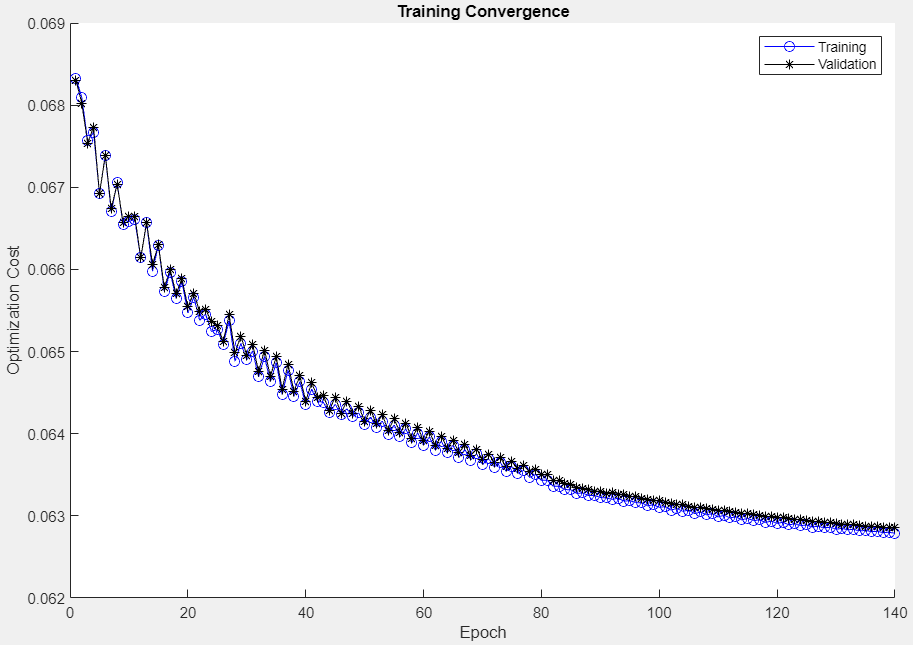
\includegraphics[height=5.5cm,keepaspectratio]{img/roll_tuning.png}
        \caption{Training convergence plot for Roll to find the iteration with the minimum training RMSE and validation RMSE}
        \label{fig:roll_tuning}
    \end{minipage}
    \hfill
    \begin{minipage}[b]{0.45\textwidth}
        \centering
        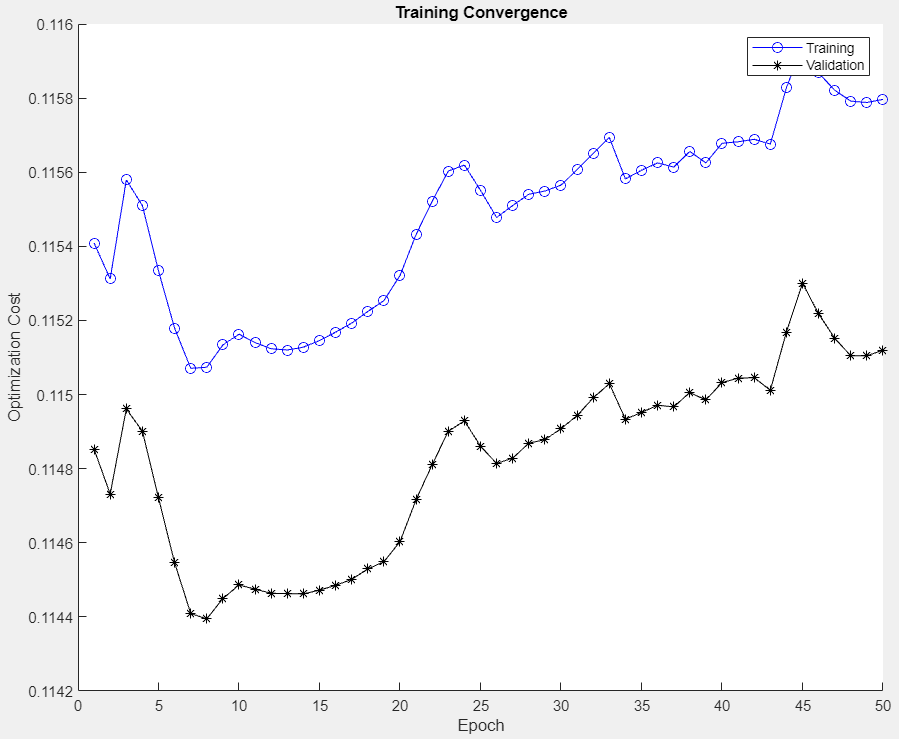
\includegraphics[height=5.5cm,keepaspectratio]{img/pitch_tuning.png}
        \caption{Training convergence plot for Pitch to find the iteration with the minimum training RMSE and validation RMSE}
        \label{fig:pitch_tuning}
    \end{minipage}
\end{figure}
\begin{figure}[H]
    \centering
    \begin{minipage}[b]{0.45\textwidth}
        \centering
        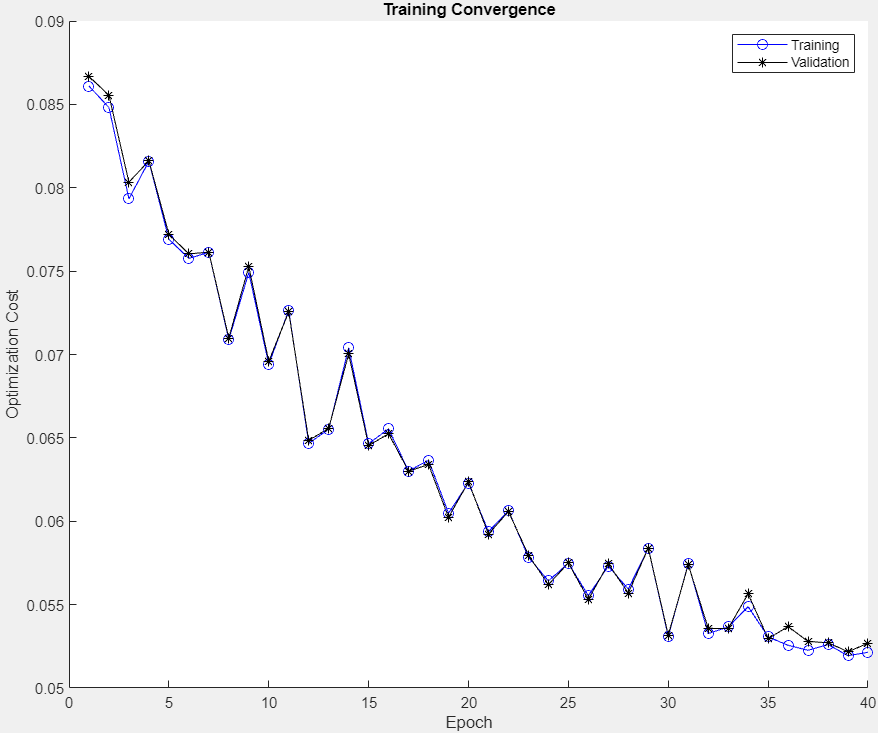
\includegraphics[height=5.5cm,keepaspectratio]{img/yaw_tuning.png}
        \caption{Training convergence plot for Yaw to find the iteration with the minimum training RMSE and validation RMSE}
        \label{fig:yaw_tuning}
    \end{minipage}
    \hfill
    \begin{minipage}[b]{0.45\textwidth}
        \centering
        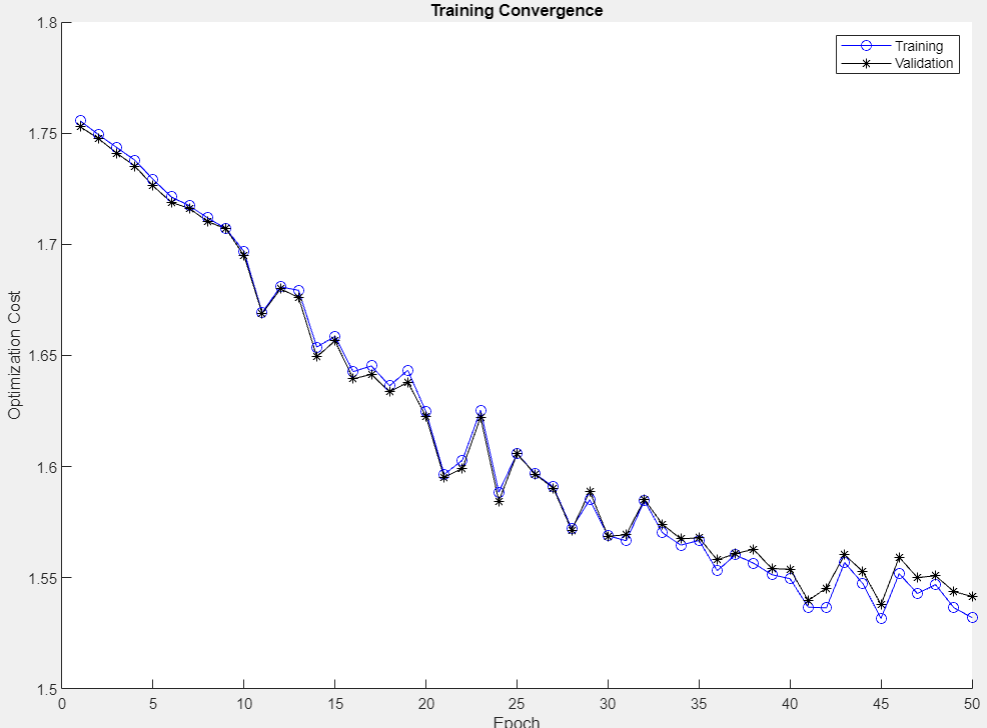
\includegraphics[height=5.5cm,keepaspectratio]{img/thrust_tuning.png}
        \caption{Training convergence plot for Thrust to find the iteration with the minimum training RMSE and validation RMSE}
        \label{fig:thrust_tuning}
    \end{minipage}
\end{figure}
The results from tuning are summarised in Table \ref{tab:results1}. The number of epochs represents the number of passes through the training dataset. As seen from Table \ref{tab:results1} and Figures \ref{fig:roll_tuning}, \ref{fig:pitch_tuning}, \ref{fig:yaw_tuning},\ref{fig:thrust_tuning}, the number of epochs were adjusted in order to allow the tuning process to reach the minimum validation error and corresponding training error. 
\begin{table}[H]
\centering
    \begin{tabular}{@{}lllll@{}}
        \toprule
                                      & Roll    & Pitch  & Yaw     & Thrust \\ \midrule
        Number of   epochs            & 140     & 50     & 60      & 50     \\
        Number of   tuning parameters & 731     & 464    & 1075    & 989    \\
        Minimum   Validation RMSE     & 0.06285 & 0.1151 & 0.04589 & 1.5380 \\
        Training RMSE                 & 0.06279 & 0.1144 & 0.04850 & 1.5317 \\ \bottomrule
    \end{tabular}
    \caption{Validation tuning results.}
    \label{tab:results1}
\end{table}
\subsection{ANFIS Parameter Selection}
After tuning, the ANFIS for each output was converted to Mamdani and Type-2 systems and then the test data was compared to the training data. The results for each `Type' were first obtained, in line with the methodology given in Figure \ref{fig:flow_fis}. RMSE was used as the performance metric to compare the configurations. The results for comparing each `Type' for each output can be seen in Table \ref{tab:results2}, with the plots in the Appendix (Figures \ref{fig:roll_type}, \ref{fig:pitch_type}, \ref{fig:yaw_type}, \ref{fig:thrust_type}). As seen, the optimal Type for all Sugeno ANFIS configurations was Type-1 in all cases. For the Mamdani configurations, the optimal type for the Roll and Yaw outputs was Type-2 and for the Pitch and Thrust outputs was Type-1.
\begin{table}[H]
\centering
    \begin{tabular}{@{}lllllllll@{}}
        \toprule
        & \multicolumn{2}{c}{Roll} & \multicolumn{2}{c}{Pitch} & \multicolumn{2}{c}{Yaw} & \multicolumn{2}{c}{Thrust} \\
        & Sugeno     & Mamdani     & Sugeno      & Mamdani     & Sugeno     & Mamdani    & Sugeno      & Mamdani      \\
        \midrule
        Optimal   “Type” & Type-1     & Type-2      & Type-1      & Type-1      & Type-1     & Type-1     & Type-1      & Type-1      \\
        \bottomrule
    \end{tabular}
    \caption{Results from comparing each configuration ``type'' for each output variable.}
    \label{tab:results2}
\end{table}
Following this, the Sugeno and Mamdani configurations were compared using the optimal ``Type'' for each (as per Table \ref{tab:results2}) and using RMSE as the performance metric for both systems. These can be seen in Figures \ref{fig:roll_SvM}, \ref{fig:pitch_SvM}, \ref{fig:yaw_SvM} and \ref{fig:thrust_SvM}. The results show that the Mamdani ANFIS has a consistent range of prediction errors whereas Sugeno fluctuate more. This is due to the Sugeno design producing crisp values for the membership function whereas Mamdani uses fuzzy sets for its membership function, meaning the Mamdani has less fluctuation in its errors. Despite this, as seen from the figures, Sugeno Type-1 was the best configuration for all four outputs as it provided the minimum RMSE in all cases. This followed what was found in the literature review as Sugeno Type-1 FIS are known for its direct, crisp output and better computational efficiency, whereas Mamdani Type-2 FIS are generally better in applications where human reasoning and non-crisp outputs are preferred \cite{zain3,boxi12}. Therefore, in the context of a drone application, where all four outputs (roll, pitch, yaw and thrust) are to be crisp and have measurable values, it was logical that the Sugeno Type-1 configuration was the best. 
\begin{figure}[H]
    \centering
    \begin{minipage}[b]{0.45\textwidth}
        \centering
        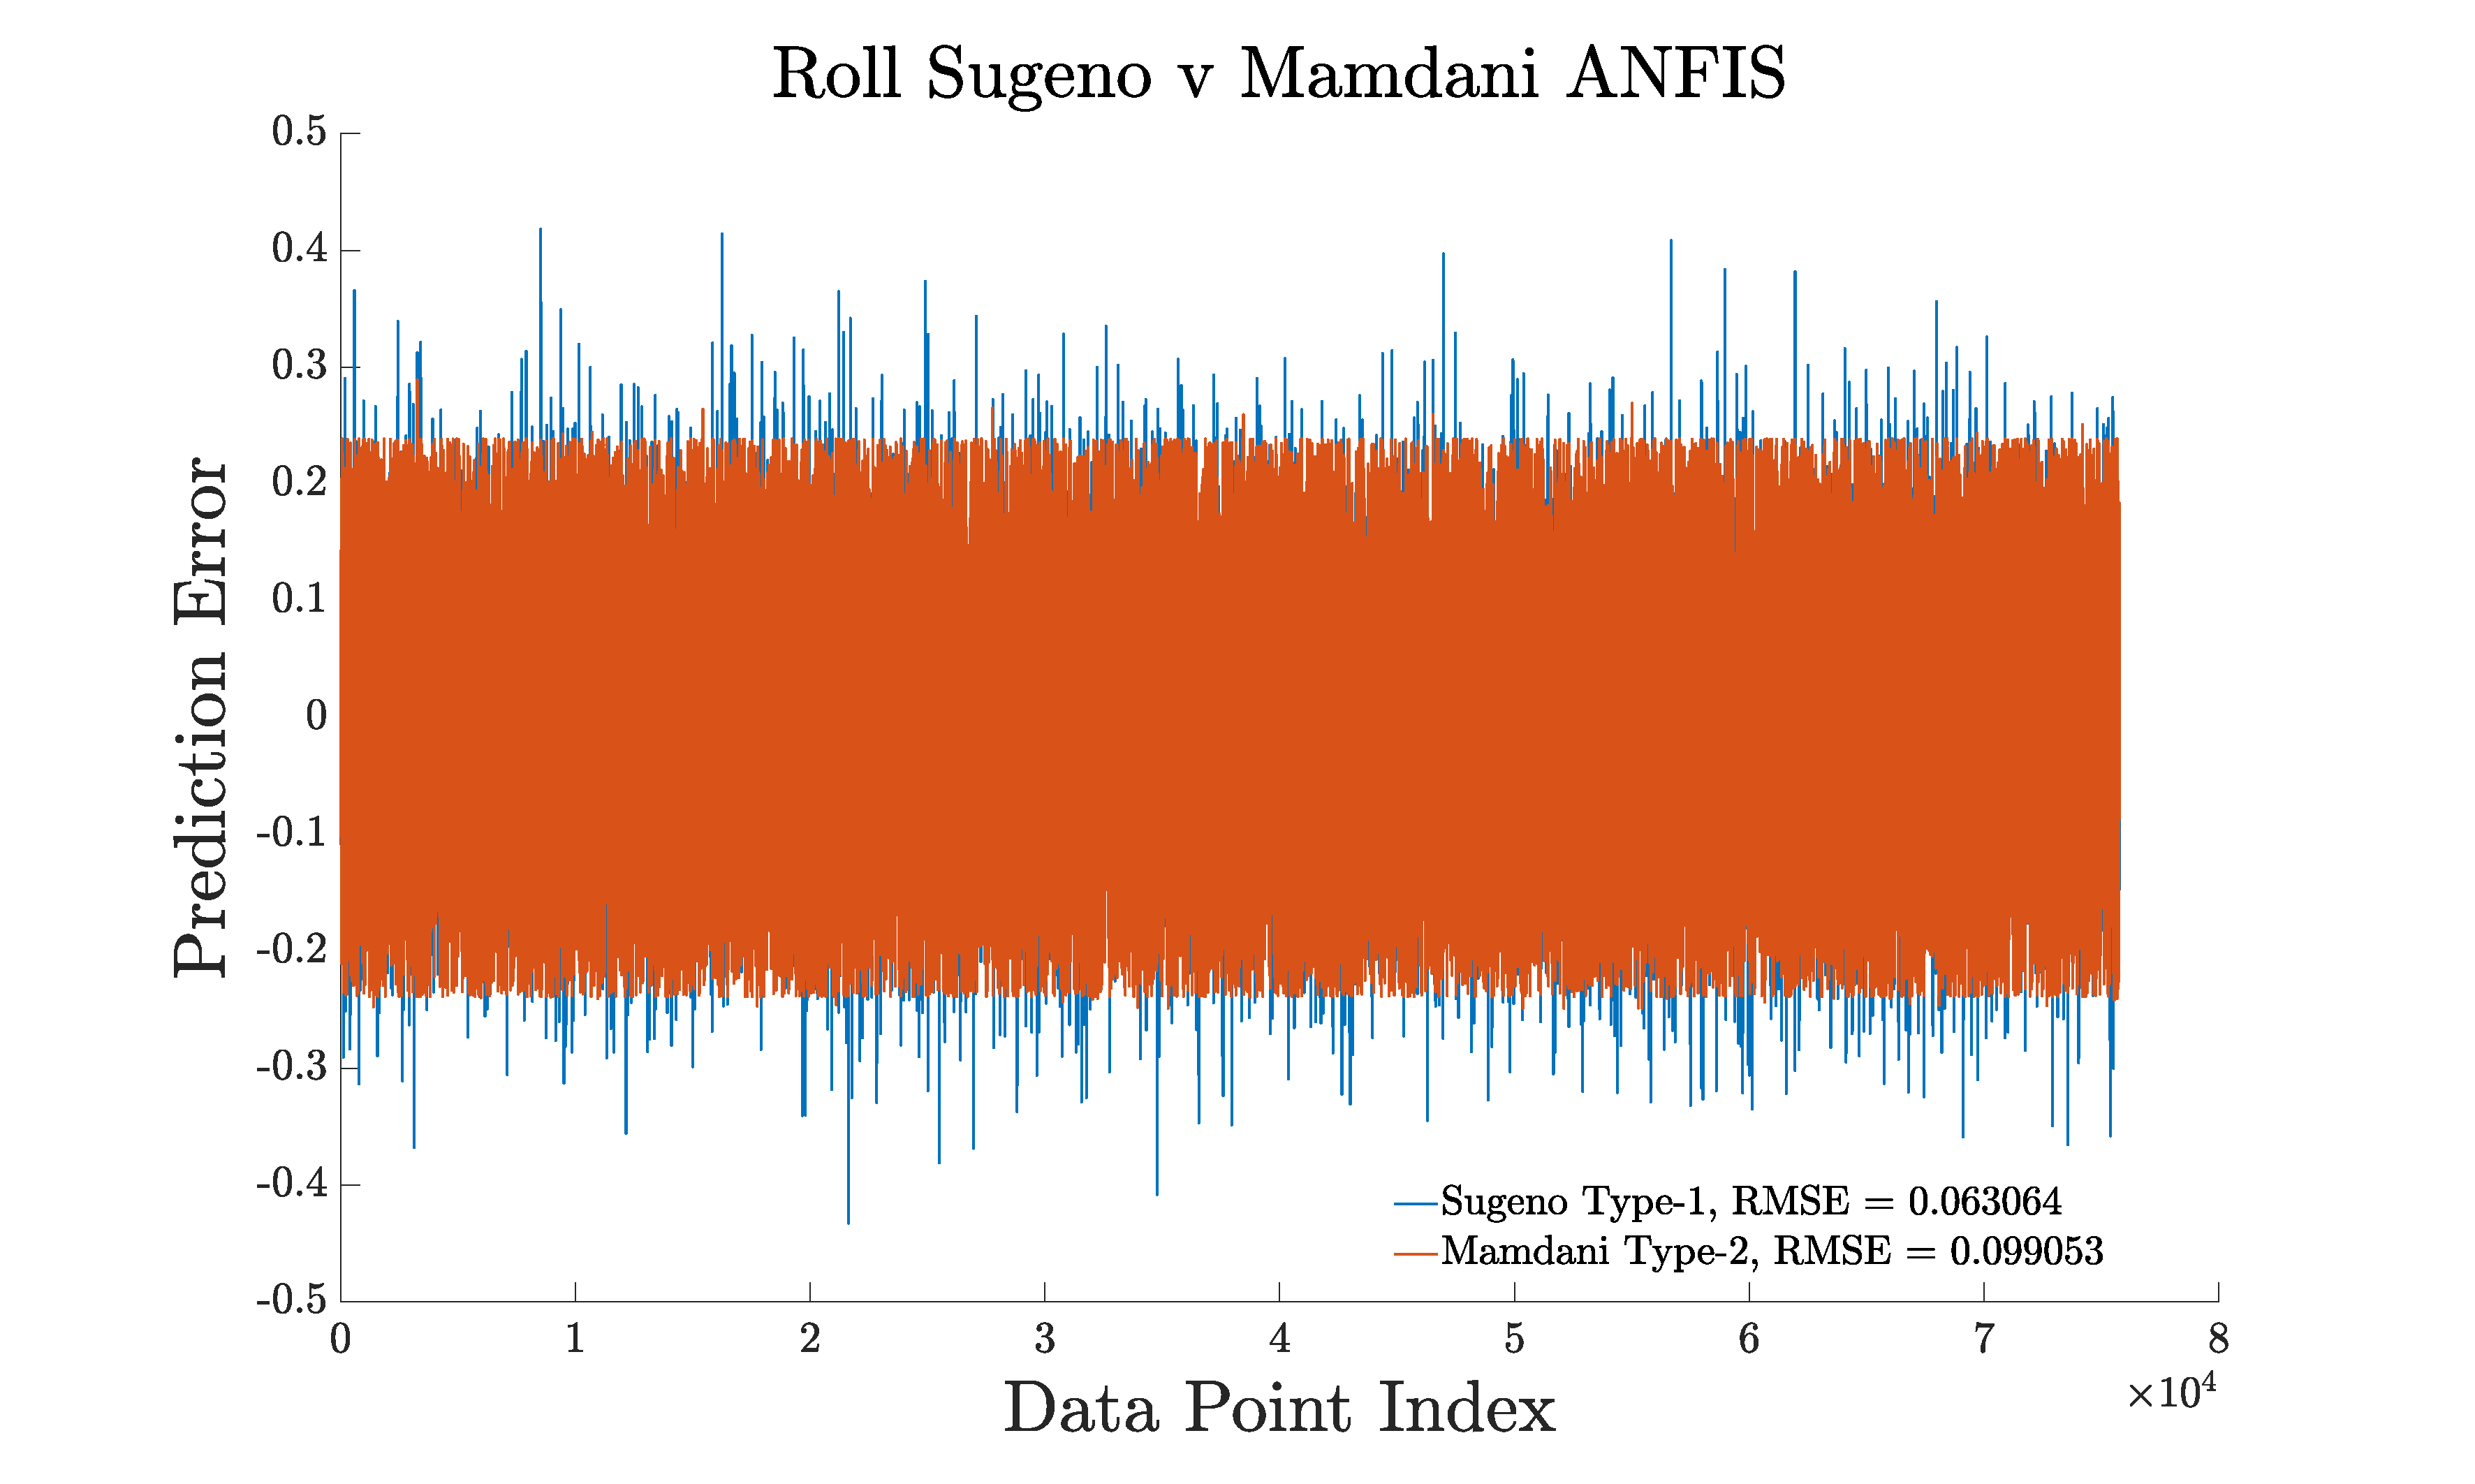
\includegraphics[height=5cm,keepaspectratio]{img/Roll SvM.pdf}
        \caption{RMSE results for the best Sugeno and Mamdani Configurations for Roll Output}
        \label{fig:roll_SvM}
    \end{minipage}
    \hfill
    \begin{minipage}[b]{0.45\textwidth}
        \centering
        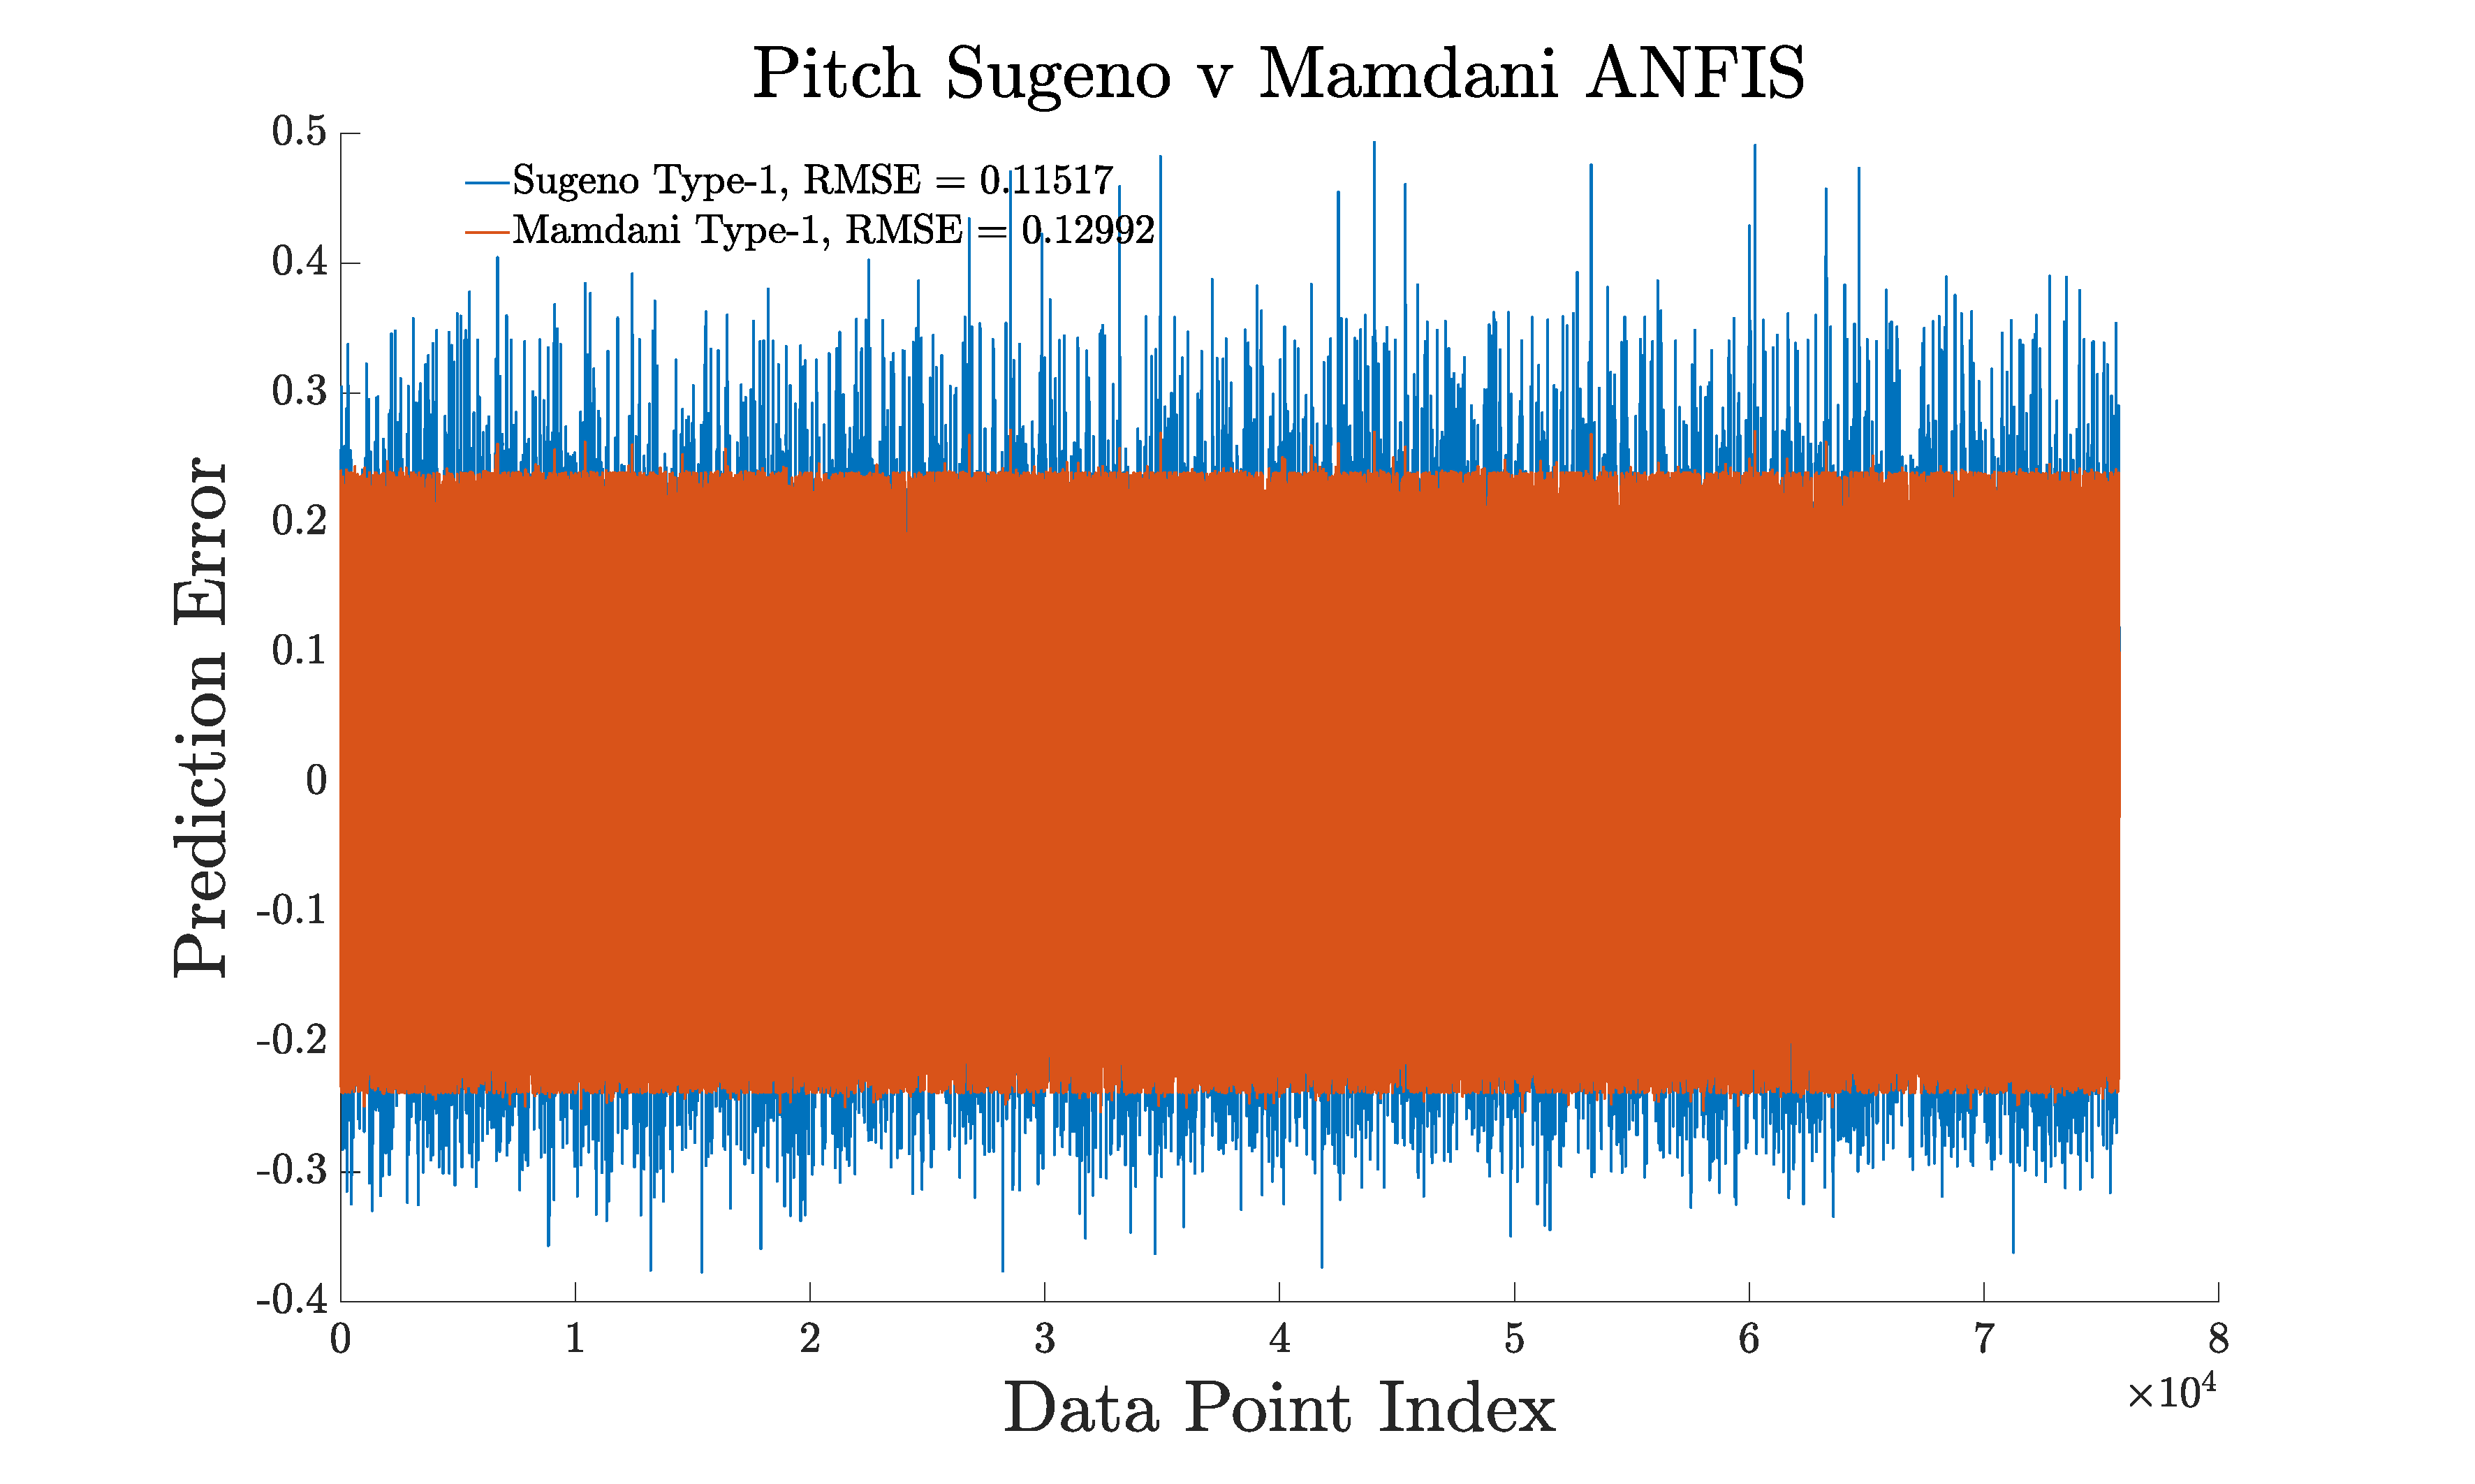
\includegraphics[height=5cm,keepaspectratio]{img/Pitch SvM.pdf}
        \caption{RMSE results for the best Sugeno and Mamdani Configurations for Pitch Output}
        \label{fig:pitch_SvM}
    \end{minipage}
\end{figure}
\begin{figure}[H]
    \centering
    \begin{minipage}[b]{0.45\textwidth}
        \centering
        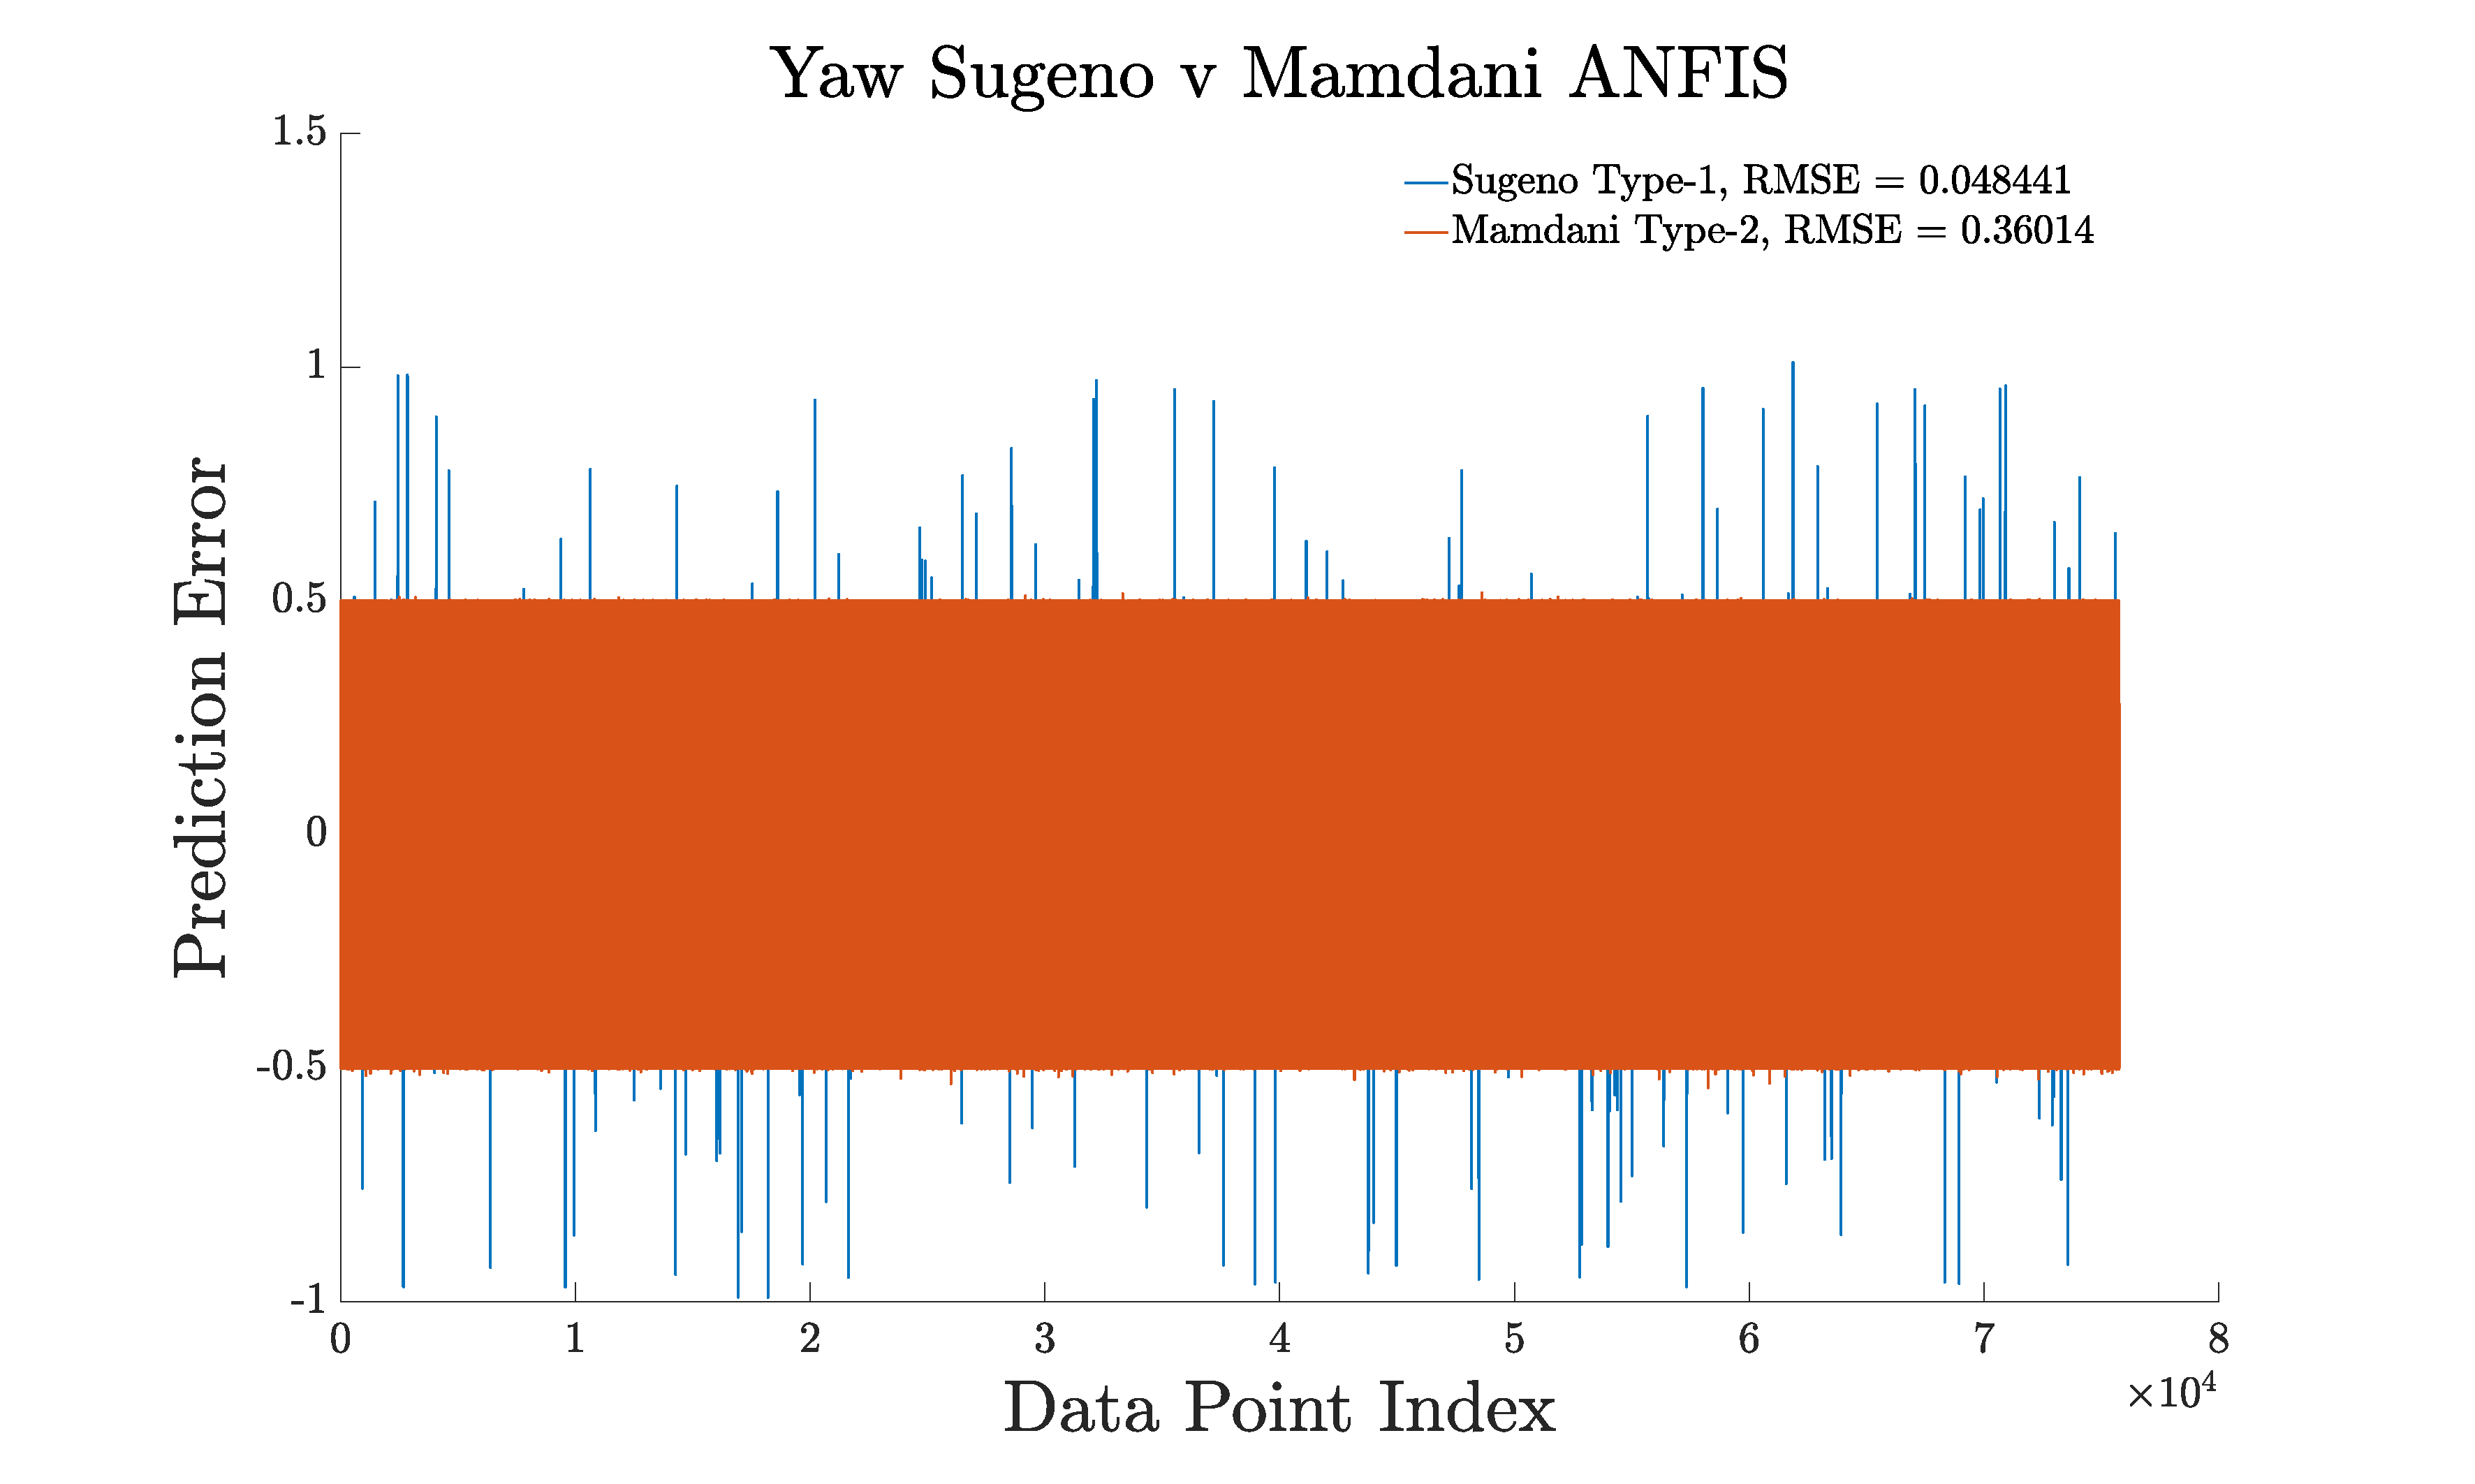
\includegraphics[height=5cm,keepaspectratio]{img/Yaw SvM.pdf}
        \caption{RMSE results for the best Sugeno and Mamdani Configurations for Yaw Output}
        \label{fig:yaw_SvM}
    \end{minipage}
    \hfill
    \begin{minipage}[b]{0.45\textwidth}
        \centering
        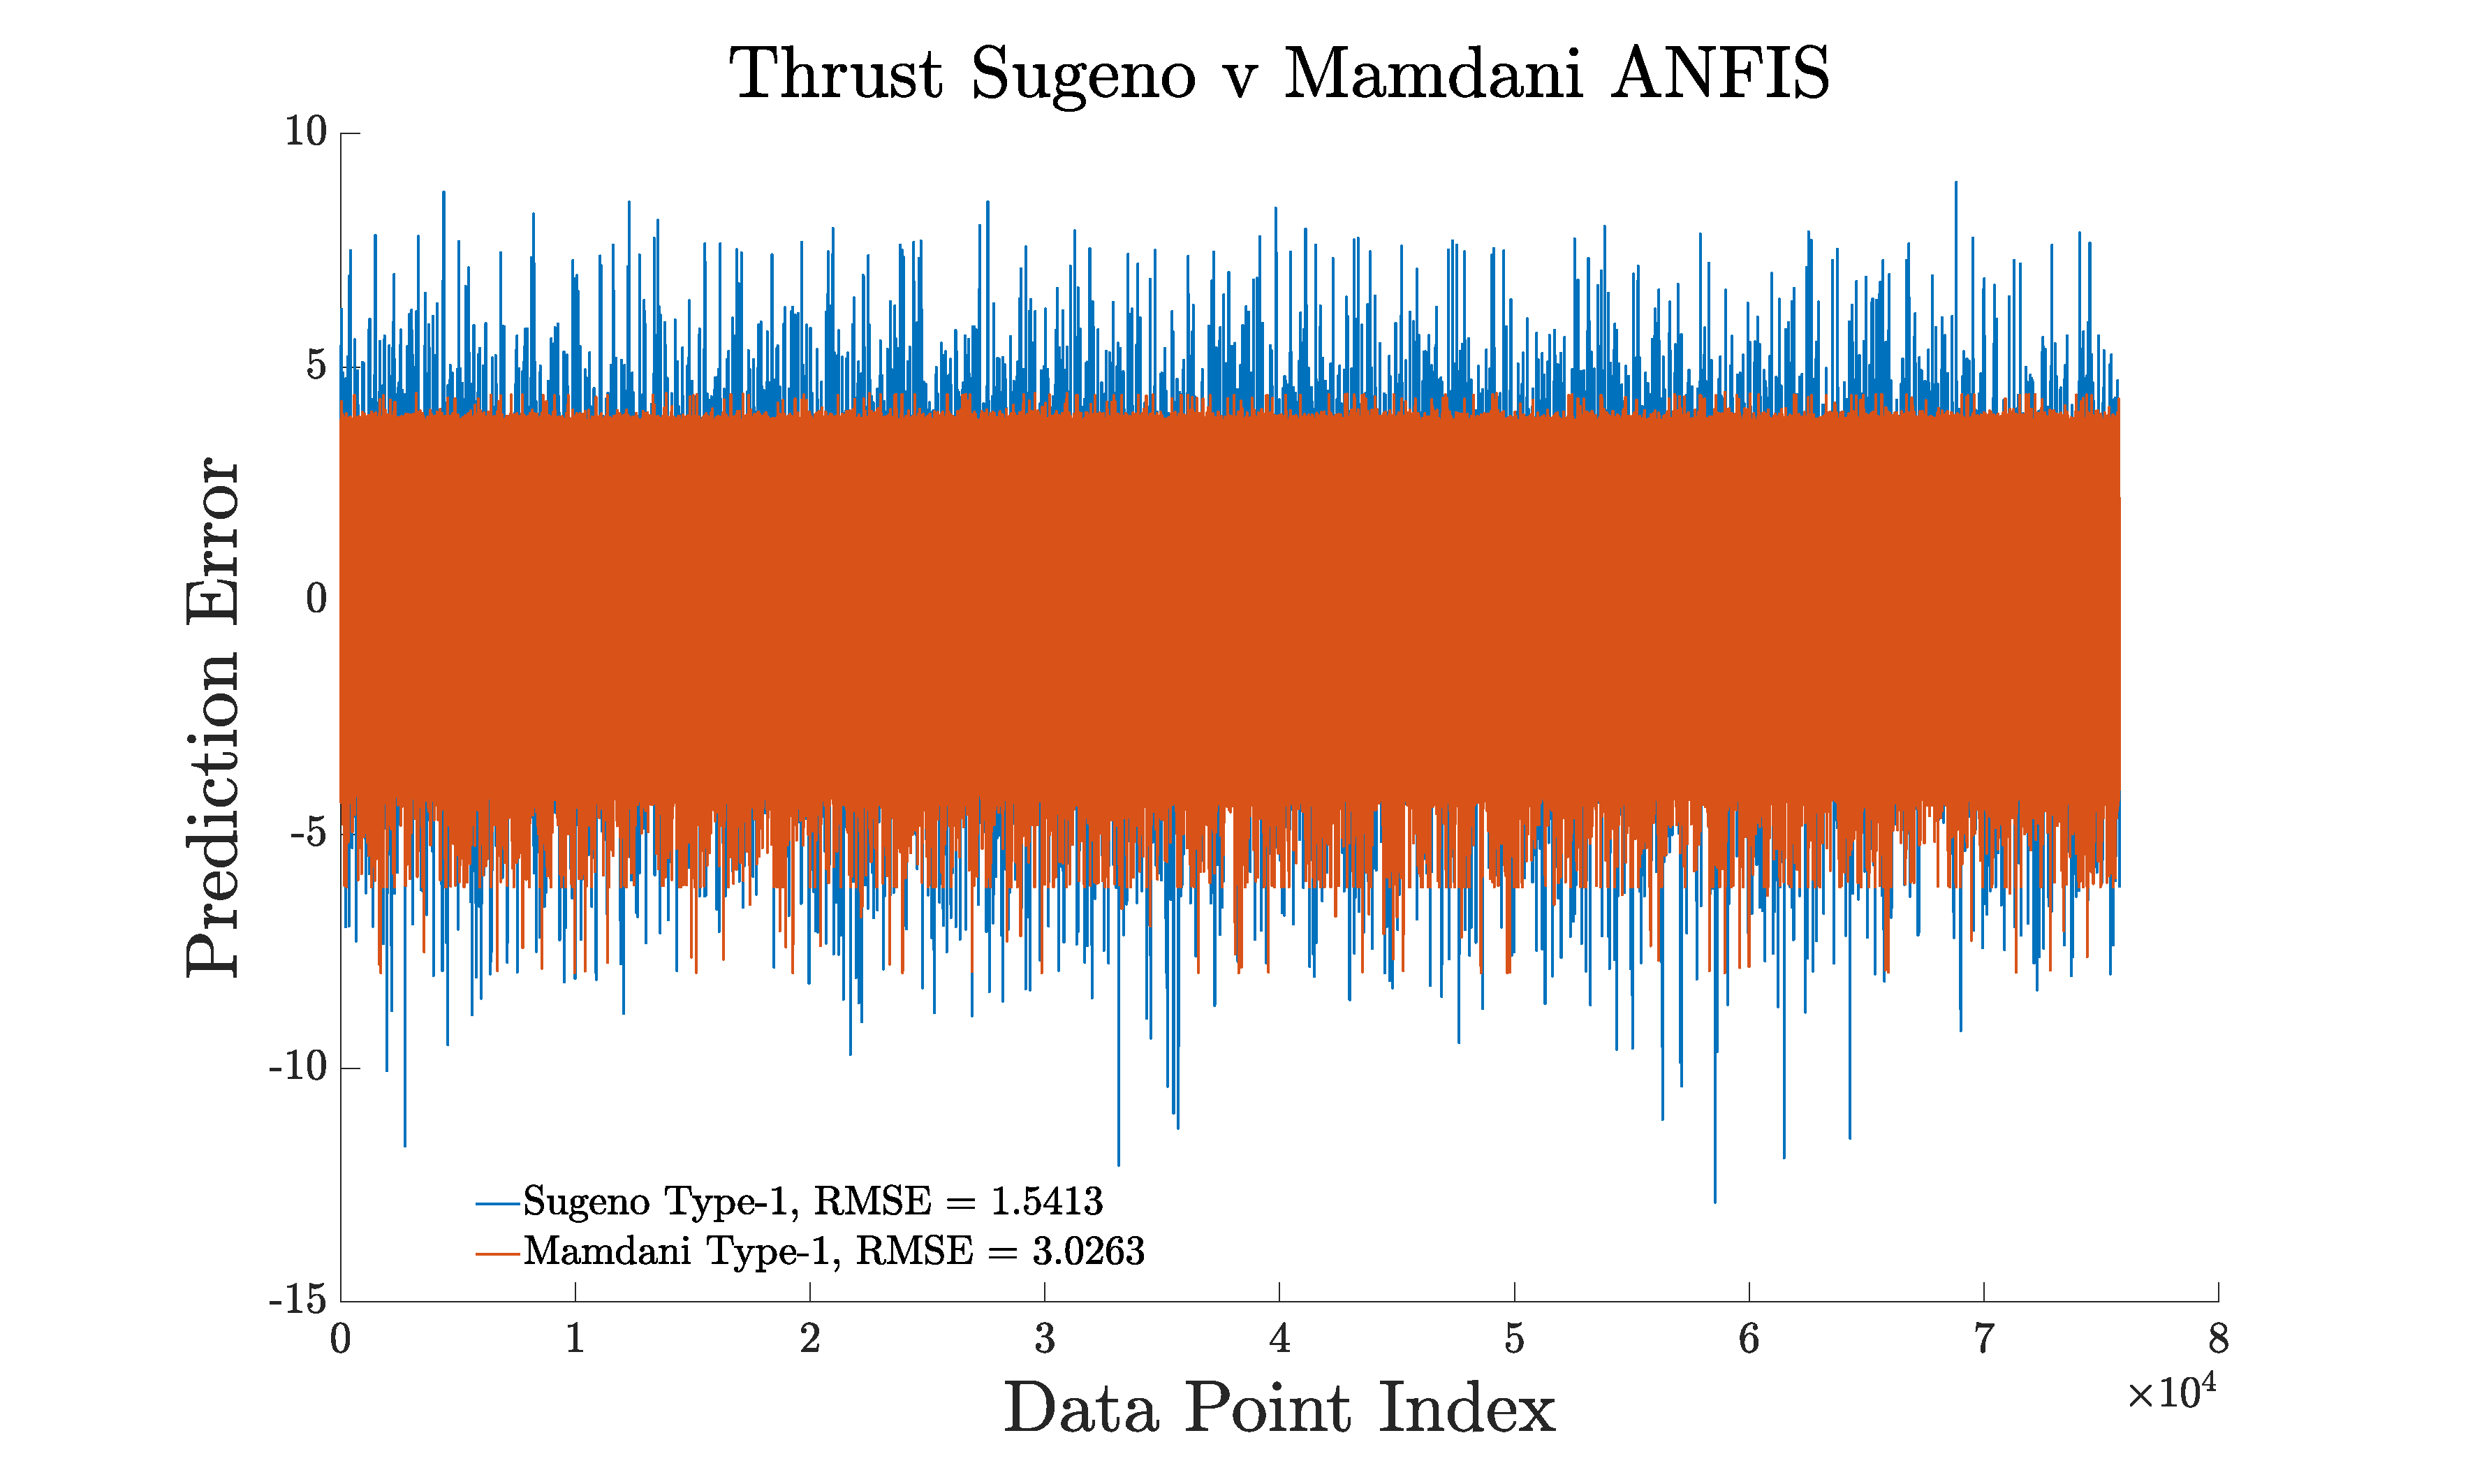
\includegraphics[height=5cm,keepaspectratio]{img/Thrust SvM.pdf}
        \caption{RMSE results for the best Sugeno and Mamdani Configurations for Thrust Output}
        \label{fig:thrust_SvM}
    \end{minipage}
\end{figure}
It was difficult to understand the performance of the models from RMSE as these are judged relative to the range of the output, therefore, the normalised RMSE was calculated. 
\begin{equation}
\text{Normalised RMSE} = \frac{\text{RMSE}}{\text{Range}}
\end{equation}
The Normalised Root Mean Square Error results of the ANFIS for each output is shown in Table \ref{tab:table_errors}. A good Normalised Root Mean Square Error (NRMSE) is highly dependent on the application. For UAV imaging, a NRMSE of 15\% or less is generally found \cite{zain4}. Table \ref{tab:table_errors} indicates that the prediction of Roll and Yaw are under this threshold at 13.2\% and 4.8\% respectively and therefore are accurate predictions. However, the thrust and especially pitch may not be as accurate as desired at 19.1\% and 24.1\% respectively. For this application, we would argue a 19.2\% NRMSE for thrust is unlikely to pose significant problems and the fact that it does not meet the 15\% found in literature is not problematic as we believe imaging prediction requires higher precision. However the 24.1\% NRMSE for Pitch could provide complications as this error is significantly higher than the 15\% seen in literature.
\begin{table}[H]
\centering
    \begin{tabular}{@{}lllll@{}}
        \toprule
        & Roll   & Pitch   & Yaw      & Thrust \\
        \midrule
        RMSE of   optimal configuration & 0.0631 & 0.11517 & 0.048441 & 1.5413 \\
        Normalised RMSE of optimal configuration & 0.1320 & 0.2411  & 0.04844  & 0.1909 \\
        \bottomrule     
    \end{tabular}
    \caption{RMSE and Normalised RMSE Errors for each output's best ANFIS Configuration}
    \label{tab:table_errors}
\end{table}
\section{Control Response Results}
Using the best ANFIS configurations found in Section 5.1, these design decisions were implemented into the simulator as shown in Figure \ref{fig:Hybrid Control}. Consequently, the simulator was tested using the PID controller and the Fuzzy Logic Controller and the error in position and computational power were compared. The scenarios are outlined in Chapter 3. (Figures \ref{fig:3_3_scenario1}, \ref{fig:3_3_scenario2}, \ref{fig:3_3_scenario3}, \ref{fig:3_3_scenario4} and \ref{fig:3_3_scenario5})

In order to evaluate the error in control response and accuracy of the controllers, the percentage error in position was calculated for each scenario as shown below. 
\begin{align}
\textrm{{Error in Position}}_{x} &= \frac{{\textrm{{Desired Position in }} x - \textrm{{Actual Position in }} x}}{{\textrm{{Desired Position in }} x}} \\
\textrm{{Error in Position}}_{y} &= \frac{{\textrm{{Desired Position in }} y - \textrm{{Actual Position in }} y}}{{\textrm{{Desired Position in }} y}} \\
\textrm{{Error in Position}}_{z} &= \frac{{\textrm{{Desired Position in }} z - \textrm{{Actual Position in }} z}}{{\textrm{{Desired Position in }} z}}\label{eq:zain1}
\end{align}

These errors in position were plotted against time to represent the control response. As the time interval was relatively small, at \SI{0.01}{\second}, the percentage error in position signal was relatively noisy therefore a moving average filter was applied. Using classical moving average filter methods \cite{zain2}, a span of 10 was used through such that an average is calculated for every second. This smoothed the control response curves and helped interpret the results. We used literature on unmanned aerial navigation to help set thresholds of error in position to analyse against. The results of a research paper by Ashraf \textit{et al} showed that their minimum average percentage error (in this case deviated from path length) was 2.19\% \cite{zain8}. After plotting our results and using this information, two threshold of 2\% and 10\% were set to analyse our plots against. The 10\% threshold was set as we thought it provided interesting insights into the speed of the two controllers towards the beginning of our simulations. 

\subsection{Scenario 1}

Scenario 1 (shown in Figure \ref{fig:3_3_scenario1}) was the most basic scenario with no obstacles, and two way-points to test the movement of the drone using each controller in open air. The control response for the error in position $x$, $y$ and $z$ against time can be seen in Figures \ref{fig:Response1x}, \ref{fig:Response1y} and \ref{fig:Response1z}. From Figures \ref{fig:Response1x} and \ref{fig:Response1y} we can see, in both cases, the PID controller has a faster response to 10\% error in position. However, for the response of error in position $x$, both the ANFIS and PID controllers reach 2\% error in position at the same time and the ANFIS controller gets to below 2\% whilst the PID maintains this error throughout the simulation. In the case of the error in position $y$, despite having a slower response to 10\% error, the ANFIS controller has a faster response to 2\% error. Both of these responses indicate that the PID controller is quicker than the ANFIS controller at the start of the simulation and then is quicker during the middle of the simulation resulting in the overall response for the ANFIS controller being better for the error in position $x$ and $y$. 

Figure \ref{fig:Response1z} shows that the ANFIS controller has large spikes in error in position $z$, compared with the PID controller which does not. This indicates anomalous control response signals due to training errors. However, despite these spikes, the drone reaches the destination in Scenario 1 quicker using the ANFIS controller compared with the PID controller. (ANFIS controller took \SI{16.18}{\second} whereas the PID controller took \SI{20.97}{\second}).
\begin{figure}[H]
    \centering
    \begin{minipage}[b]{0.45\textwidth}
        \centering
        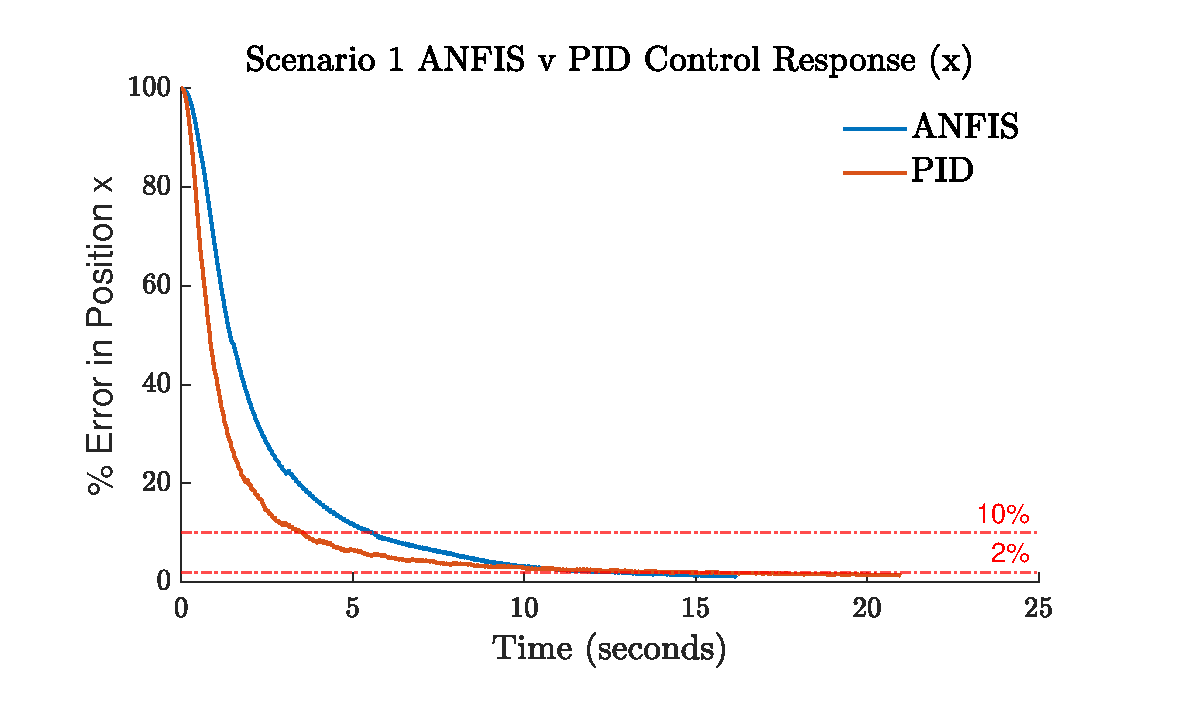
\includegraphics[height=5cm,keepaspectratio]{img/Scenario 1 Error in x Position.pdf}
        \caption{Scenario 1 Control Response (Error between Desired position $x$ and Actual position $x$) for PID and ANFIS Control}
        \label{fig:Response1x}
    \end{minipage}
    \hfill
    \begin{minipage}[b]{0.45\textwidth}
        \centering
        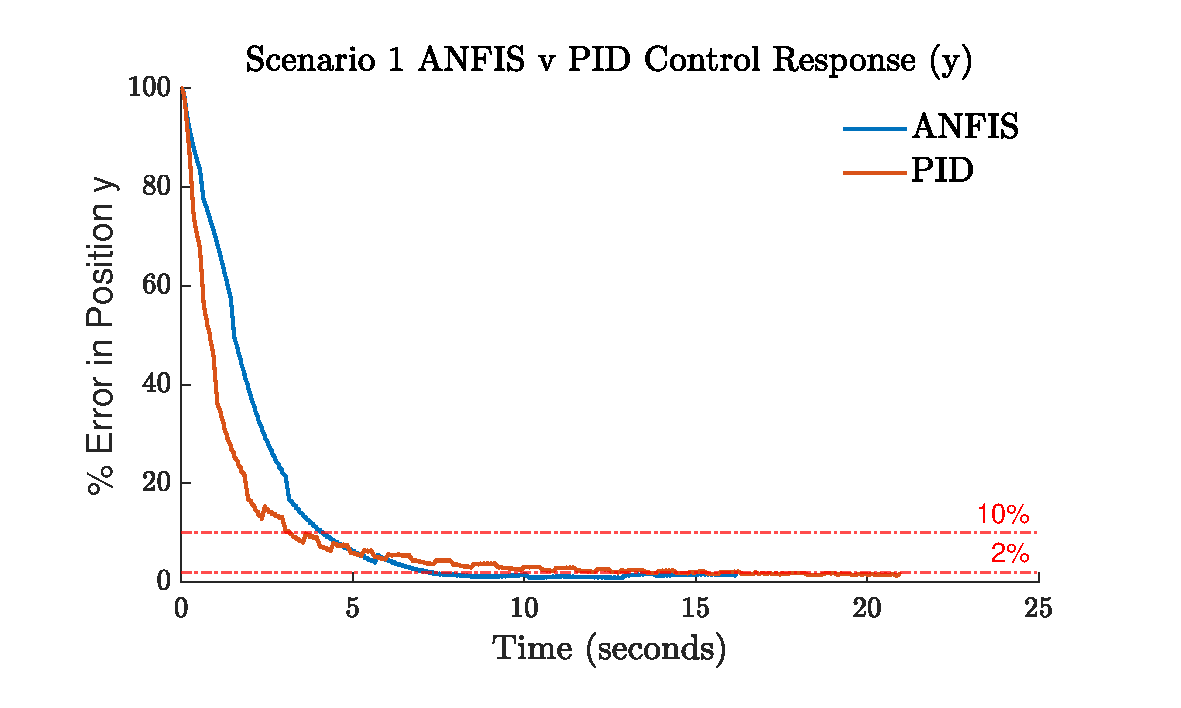
\includegraphics[height=5cm,keepaspectratio]{img/Scenario 1 Error in y Position.pdf}
        \caption{Scenario 1 Control Response (Error between Desired position $y$ and Actual position $y$) for PID and ANFIS Control}
        \label{fig:Response1y}
    \end{minipage}
\end{figure}
\begin{figure}[H]
    \centering
    \begin{minipage}[b]{0.45\textwidth}
        % empty minipage
    \end{minipage}
    \hfill
    \begin{minipage}[b]{0.45\textwidth}
        \centering
        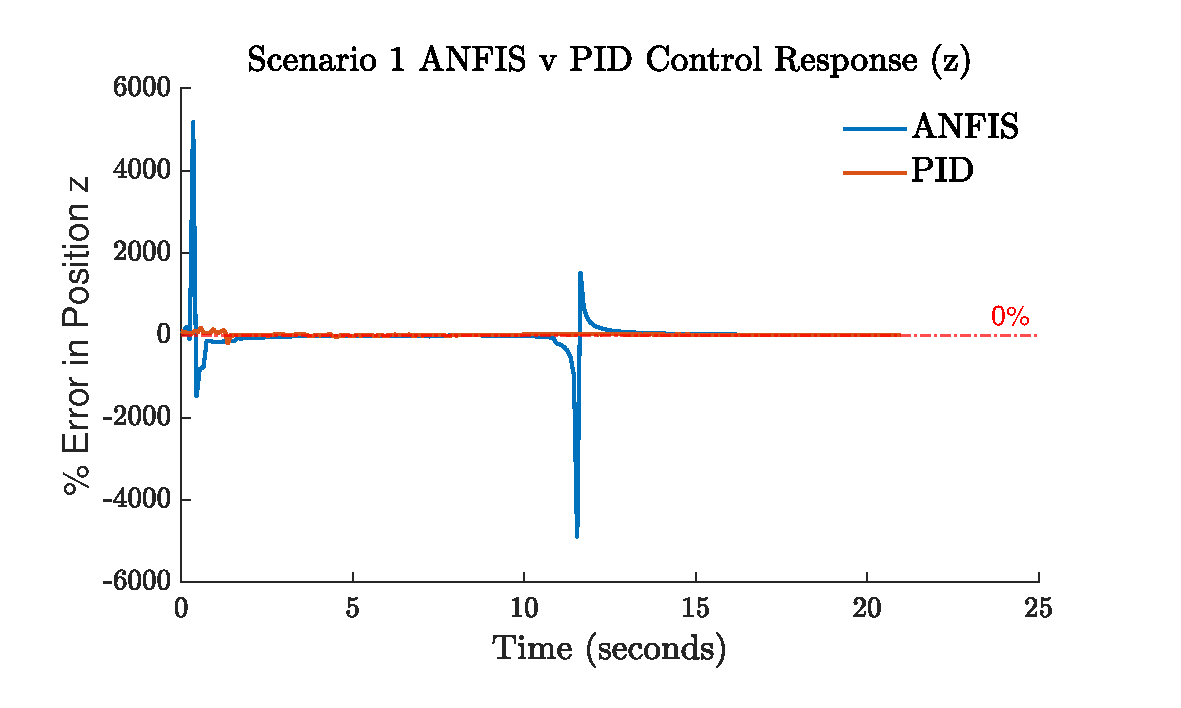
\includegraphics[height=5cm,keepaspectratio]{img/Scenario 1 Error in z Position.pdf}
        \caption{Scenario 1 Control Response (Error between Desired position $z$ and Actual position $z$) for PID and ANFIS Control}
        \label{fig:Response1z}
    \end{minipage}
    \hfill
    \begin{minipage}[b]{0.45\textwidth}
        % empty minipage
    \end{minipage}
\end{figure}

\subsection{Scenario 2}

Scenario 2 (shown in Figure \ref{fig:3_3_scenario2}) was another basic scenario with only two obstacles, both short in height and width, and one of which obstructed the path of the drone. The control response for the error in position $x$, $y$ and $z$ against time can be seen in Figures \ref{fig:Response2x}, \ref{fig:Response2y} and \ref{fig:Response2z}. Figures \ref{fig:Response2x} and \ref{fig:Response2y} shows that the PID controller has a faster response than the ANFIS controller to the 10\% error threshold in both the error in position $x$ and $y$. However, the ANFIS controller's response is quicker below this 10\% threshold meaning the ANFIS controller reaches the 2\% threshold faster than the PID controller in both cases. 

Similar to Scenario 1, Figure \ref{fig:Response2z} shows the ANFIS controller has a spike in $z$ position which similarly is likely to be caused by a training error causing an anomalous response. As the pitch output had the largest normalised RMSE (see Table \ref{tab:table_errors}), an error in this FIS is likely to have caused this anamolous response. However, despite this, the ANFIS controller again reaches its destination 29.2\% quicker due to its faster response in positions $x$ and $y$. 

\begin{figure}[H]
    \centering
    \begin{minipage}[b]{0.45\textwidth}
        \centering
        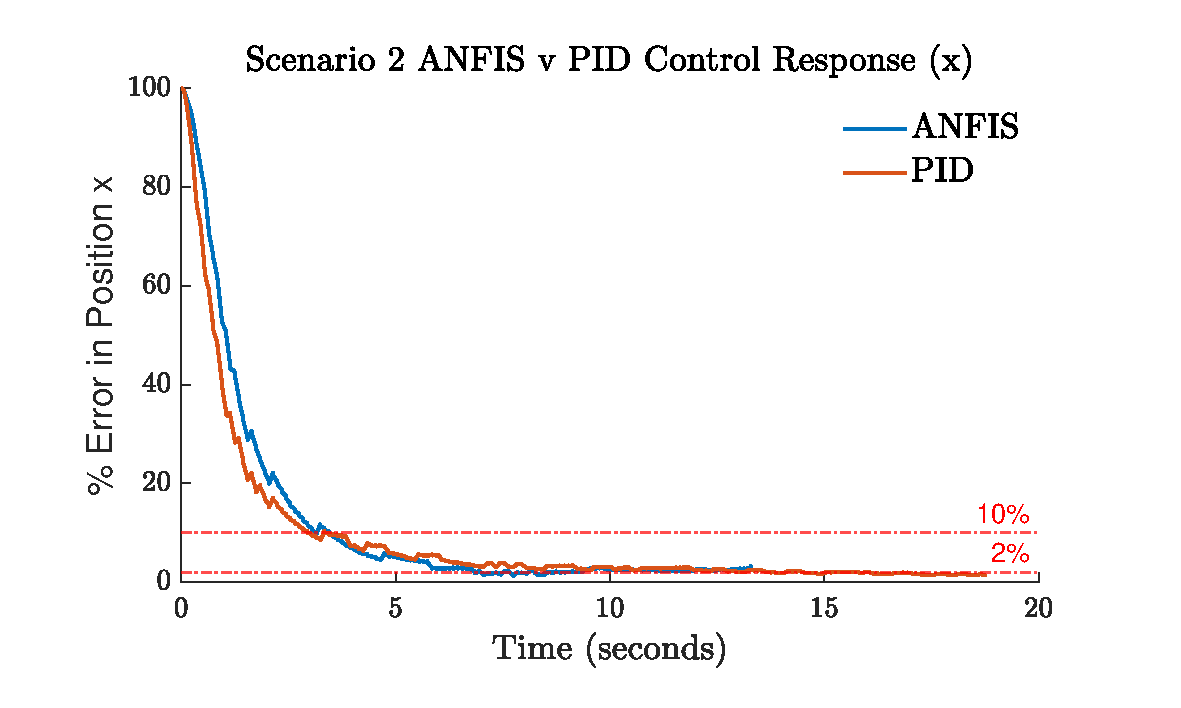
\includegraphics[height=5cm,keepaspectratio]{img/Scenario 2 Error in x Position.pdf}
        \caption{Scenario 2 Control Response (Error between Desired position $x$ and Actual position $x$) for PID and ANFIS Control}
        \label{fig:Response2x}
    \end{minipage}
    \hfill
    \begin{minipage}[b]{0.45\textwidth}
        \centering
        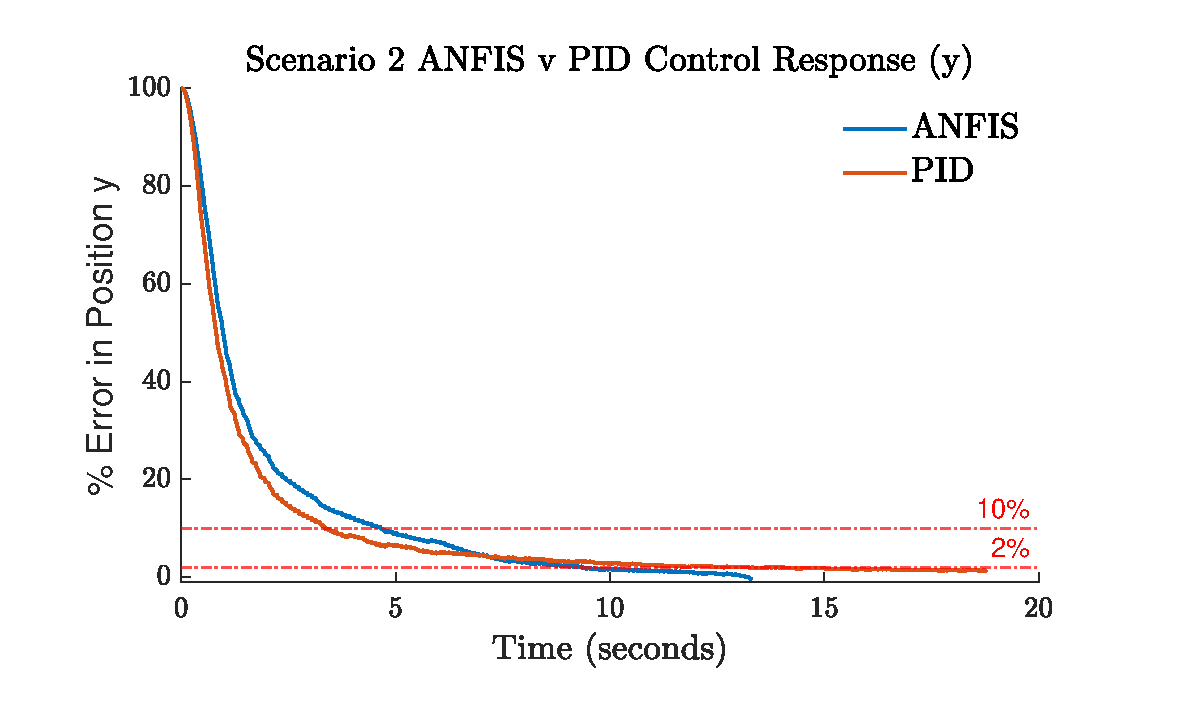
\includegraphics[height=5cm,keepaspectratio]{img/Scenario 2 Error in y Position.pdf}
        \caption{Scenario 2 Control Response (Error between Desired position $y$ and Actual position $y$) for PID and ANFIS Control}
        \label{fig:Response2y}
    \end{minipage}
\end{figure}

\begin{figure}[H]
    \centering
    \begin{minipage}[b]{0.45\textwidth}
        % empty minipage
    \end{minipage}
    \hfill
    \begin{minipage}[b]{0.45\textwidth}
        \centering
        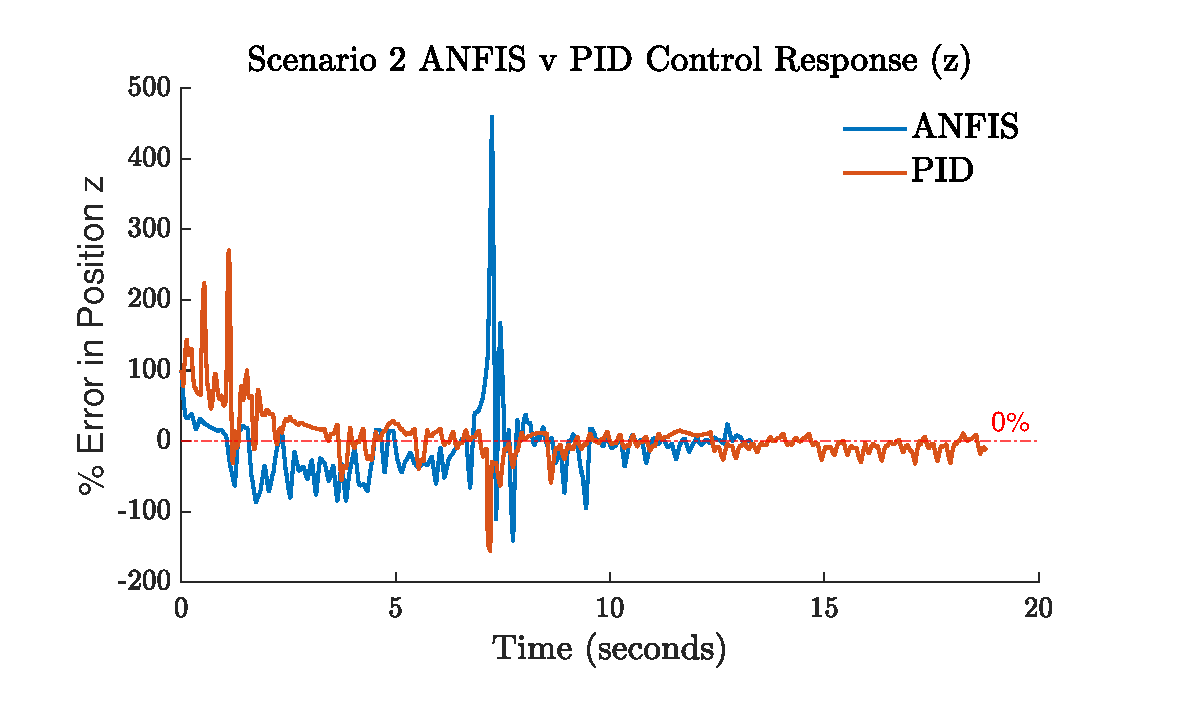
\includegraphics[height=5cm,keepaspectratio]{img/Scenario 2 Error in z Position.pdf}
        \caption{Scenario 2 Control Response (Error between Desired position $z$ and Actual position $z$) for PID and ANFIS Control}
        \label{fig:Response2z}
    \end{minipage}
    \hfill
    \begin{minipage}[b]{0.45\textwidth}
        % empty minipage
    \end{minipage}
\end{figure}

\subsection{Scenario 3}

Scenario 3 (shown in Figure \ref{fig:3_3_scenario3}) was a more challenging scenario than 1 and 2 as it tested the drones ability to go over an obstacle and therefore its ability to ascend and descend. The control response for the error in position $x$, $y$ and $z$ against time can be seen in Figures \ref{fig:Response3x}, \ref{fig:Response3y} and \ref{fig:Response3z}. Figures \ref{fig:Response3x} and \ref{fig:Response3y} shows, similar to Scenario 1 and 2, that the response of the PID controller to 10\% error in position was quicker. In this case, the PID and ANFIS response for error in position $x$ and $y$ both reach the 2\% threshold at a similar rate. 

Analogous to Scenario 1 and 2, there is a small spike in error in $z$ position, seen in \ref{fig:Response3z}, to 130\% for the ANFIS controller at the start of the simulation. Despite this spike, the ANFIS controller reaches the 10\% threshold quicker than the PID controller. However, the ANFIS controller is then slower than the PID controller to reach the 2\% threshold. The spike in error in $z$ position, as well as the slower response results in the ANFIS controller taking a longer time to reach its destination for Scenario 3. This is logically coherent with the fact that Scenario 3 was based on the drones ascending and descending movement, i.e. its $z$ position. 

\begin{figure}[H]
    \centering
    \begin{minipage}[b]{0.45\textwidth}
        \centering
        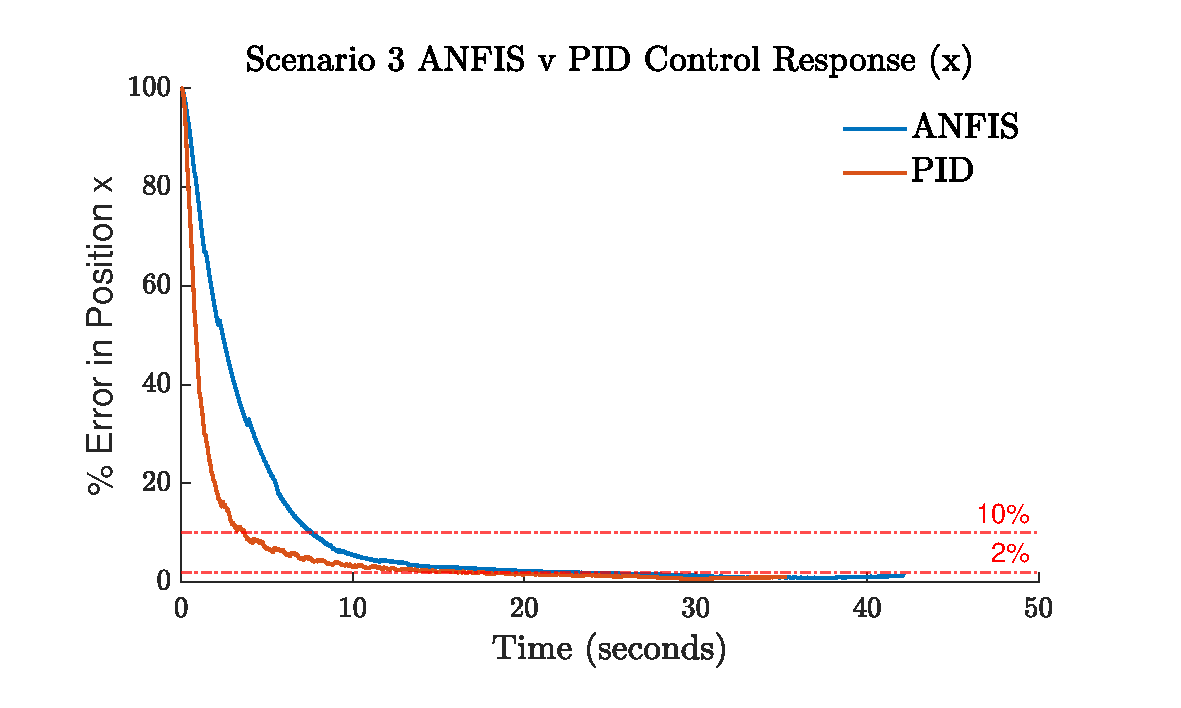
\includegraphics[height=5cm,keepaspectratio]{img/Scenario 3 Error in x Position.pdf}
        \caption{Scenario 3 Control Response (Error between Desired position $x$ and Actual position $x$) for PID and ANFIS Control}
        \label{fig:Response3x}
    \end{minipage}
    \hfill
    \begin{minipage}[b]{0.45\textwidth}
        \centering
        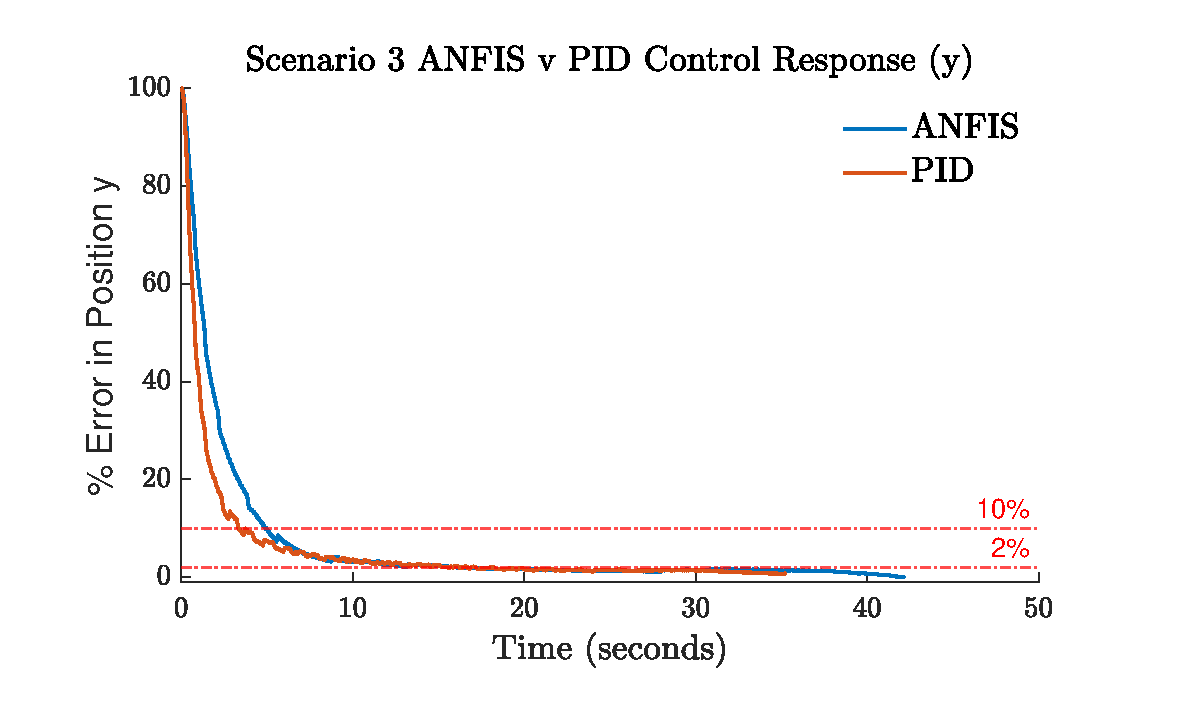
\includegraphics[height=5cm,keepaspectratio]{img/Scenario 3 Error in y Position.pdf}
        \caption{Scenario 3 Control Response (Error between Desired position $y$ and Actual position $y$) for PID and ANFIS Control}
        \label{fig:Response3y}
    \end{minipage}
\end{figure}

\begin{figure}[H]
    \centering
    \begin{minipage}[b]{0.45\textwidth}
        % empty minipage
    \end{minipage}
    \hfill
    \begin{minipage}[b]{0.45\textwidth}
        \centering
        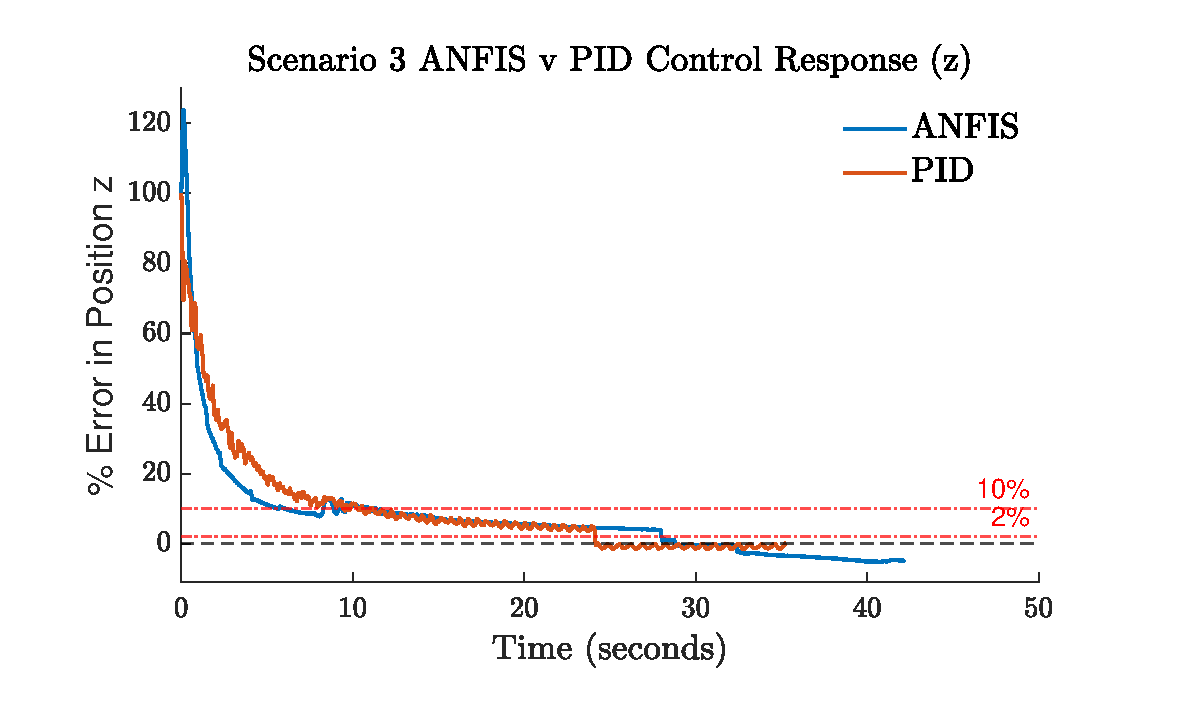
\includegraphics[height=5cm,keepaspectratio]{img/Scenario 3 Error in z Position.pdf}
        \caption{Scenario 3 Control Response (Error between Desired position $z$ and Actual position $z$) for PID and ANFIS Control}
        \label{fig:Response3z}
    \end{minipage}
    \hfill
    \begin{minipage}[b]{0.45\textwidth}
        % empty minipage
    \end{minipage}
\end{figure}

\subsection{Scenario 4}

Scenario 4 (shown in Figure \ref{fig:3_3_scenario4}) was a more challenging version of scenario 2 with another way-point added and a change of height in the way-points. The control response for the error in position $x$, $y$ and $z$ against time can be seen in Figures \ref{fig:Response4x}, \ref{fig:Response4y} and \ref{fig:Response4z}. Figures \ref{fig:Response4x} and \ref{fig:Response4y} shows, much like the trend seen from the previous scenarios, that the response of the PID controller to 10\% error in position was quicker. In this case, the PID and ANFIS response for error in position $x$ and $y$ again both reach the 2\% threshold at a similar rate, however the ANFIS controller briefly spikes to just over 3\% later in the simulation, indicating a sub-optimal response given at this point. 

In line with Scenario 4, there is a small spike in error in $z$ position, seen in \ref{fig:Response3z}, to around 130\% for the ANFIS controller at the start of the simulation. Resembling Scenario 3, despite this spike, the ANFIS controller reaches the 10\% threshold quicker than the PID controller but is then slower than the PID controller to reach the 2\% threshold. Therefore, although the ANFIS controller had an overall better control response in Scenario 2, by adding another way point that caused the drone to have to change height (change in $z$ position) in Scenario 4, the drone with an ANFIS controller then had an overall worse response in this scenario. As a result, this scenario provides interesting insight into the ANFIS controller's weakness in its change in $z$ position.
\begin{figure}[H]
    \centering
    \begin{minipage}[b]{0.45\textwidth}
        \centering
        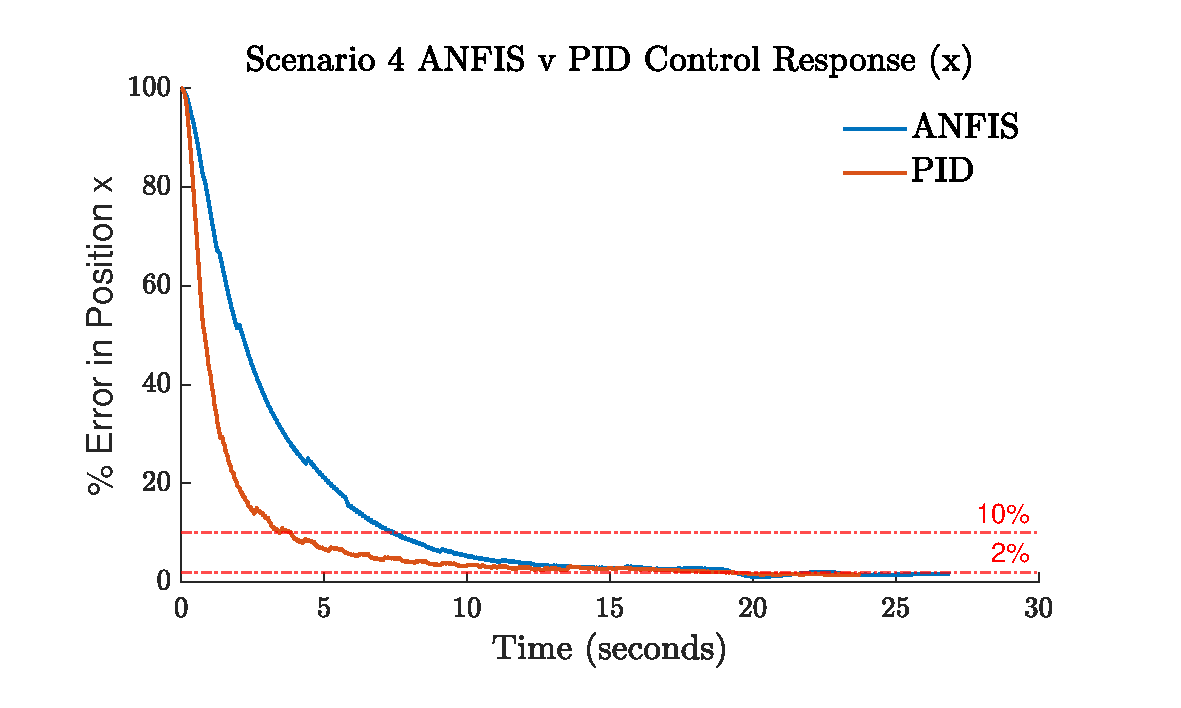
\includegraphics[height=5cm,keepaspectratio]{img/Scenario 4 Error in x Position.pdf}
        \caption{Scenario 4 Control Response (Error between Desired position $x$ and Actual position $x$) for PID and ANFIS Control}
        \label{fig:Response4x}
    \end{minipage}
    \hfill
    \begin{minipage}[b]{0.45\textwidth}
        \centering
        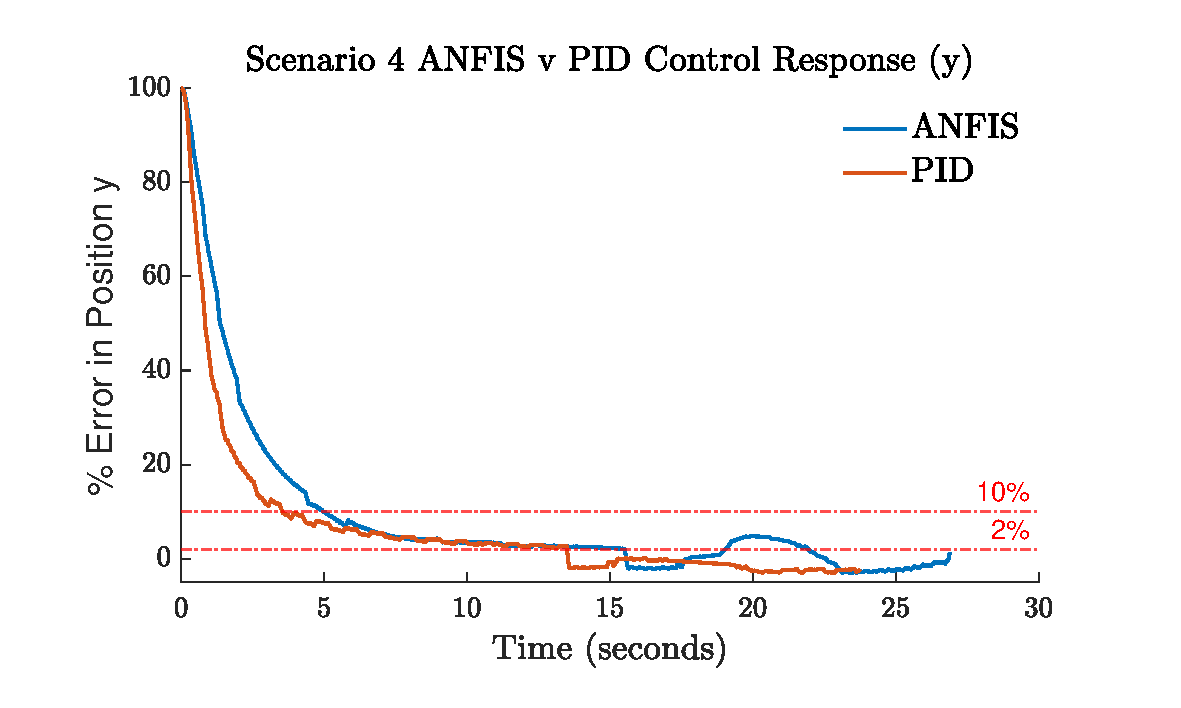
\includegraphics[height=5cm,keepaspectratio]{img/Scenario 4 Error in y Position.pdf}
        \caption{Scenario 4 Control Response (Error between Desired position $y$ and Actual position $y$) for PID and ANFIS Control}
        \label{fig:Response4y}
    \end{minipage}
\end{figure}

\begin{figure}[H]
    \centering
    \begin{minipage}[b]{0.45\textwidth}
        % empty minipage
    \end{minipage}
    \hfill
    \begin{minipage}[b]{0.45\textwidth}
        \centering
        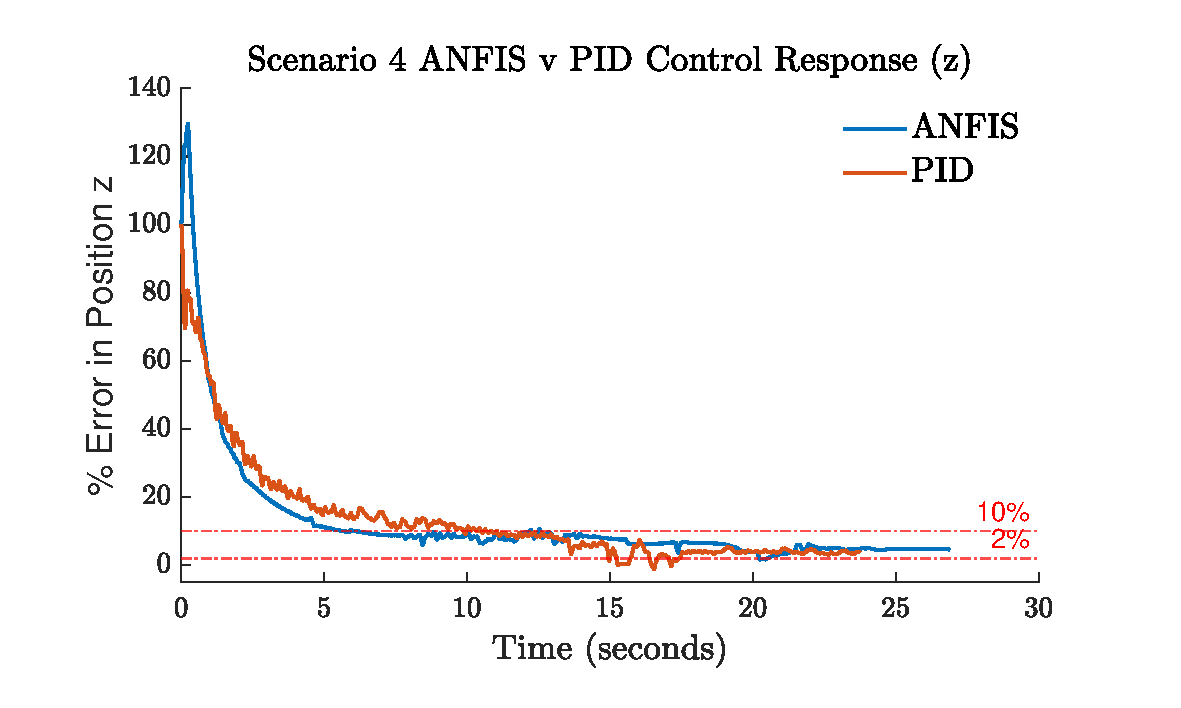
\includegraphics[height=5cm,keepaspectratio]{img/Scenario 4 Error in z Position.pdf}
        \caption{Scenario 4 Control Response (Error between Desired position $z$ and Actual position $z$) for PID and ANFIS Control}
        \label{fig:Response4z}
    \end{minipage}
    \hfill
    \begin{minipage}[b]{0.45\textwidth}
        % empty minipage
    \end{minipage}
\end{figure}

\subsection{Scenario 5}
Scenario 5 (shown in Figure \ref{fig:3_3_scenario5}) had five obstacles, one of which obstructed the path of the drone, with two way-points both at the same height. This scenario aims to test the drone's ability to operate in compact spaces, using obstacle avoidance, but does not require any significant change in height (unless needed to avoid obstacle). Figures \ref{fig:Response5x} and \ref{fig:Response5y} align with the trend seen from the previous scenarios, that the response of the PID controller to 10\% error in position was faster. The PID and ANFIS response for error in position $y$ both reach the 2\% threshold at a similar rate however the ANFIS response reaches a lower error (ANFIS reaches minimum of 0.23\% error whereas PID reaches minimum of 0.78\% error). For the error in position $x$, the PID response for the error reaches the 2\% threshold quicker. 

Figure \ref{fig:Response5z} shows that for the error in position $z$ both responses are noisy. The PID response has multiple spikes and a highly noisy response compared with the ANFIS controller which has fewer spikes and a less noisy response, These responses are likely to be noisy as the desired position $z$ is near zero, therefore any small changes in actual $z$ will result in a very large error in position $z$ (as in \eqref{eq:zain1} desired $z$ position is the denominator). 

Despite the superior performance not clearly shown in Figures \ref{fig:Response5x} \ref{fig:Response5y} and \ref{fig:Response5z}, the drone using the ANFIS controller reaches its destination 23.8\% quicker, indicating the overall control response is better. Therefore, this supports the trend that the ANFIS controller performs better in scenarios with little change in $z$ position. 
\begin{figure}[H]
    \centering
    \begin{minipage}[b]{0.45\textwidth}
        \centering
        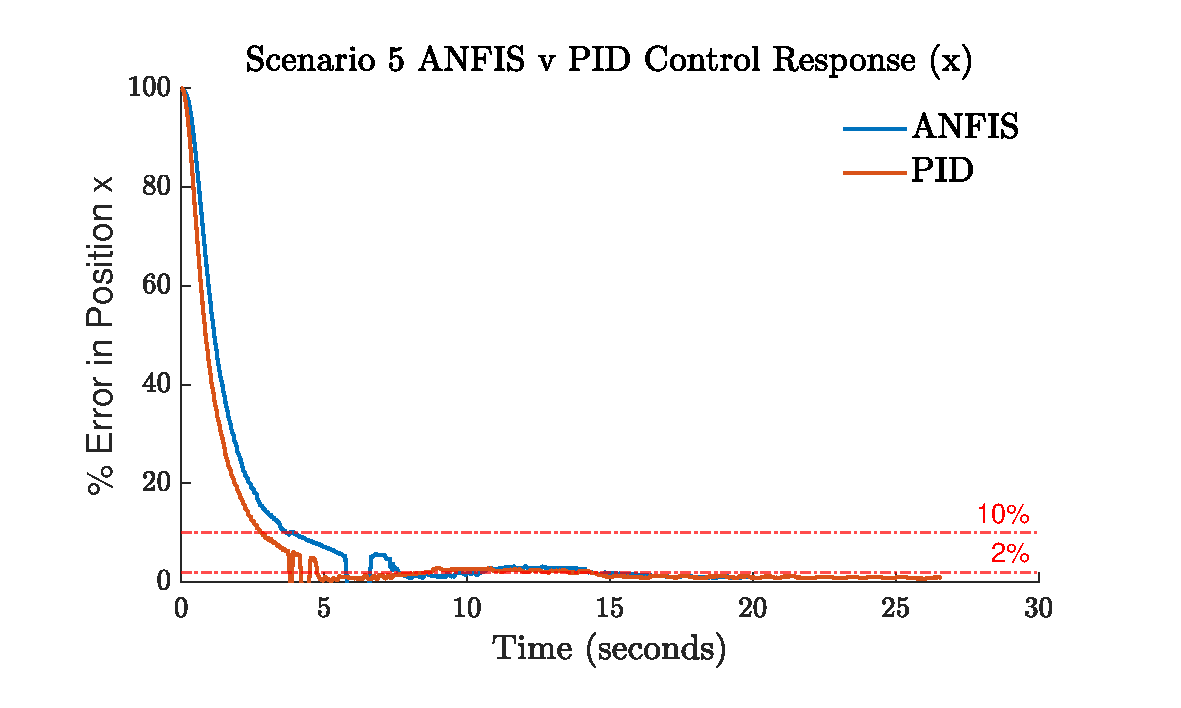
\includegraphics[height=5cm,keepaspectratio]{img/Scenario 5 Error in x Position.pdf}
        \caption{Scenario 5 Control Response (Error between Desired position $x$ and Actual position $x$) for PID and ANFIS Control}
        \label{fig:Response5x}
    \end{minipage}
    \hfill
    \begin{minipage}[b]{0.45\textwidth}
        \centering
        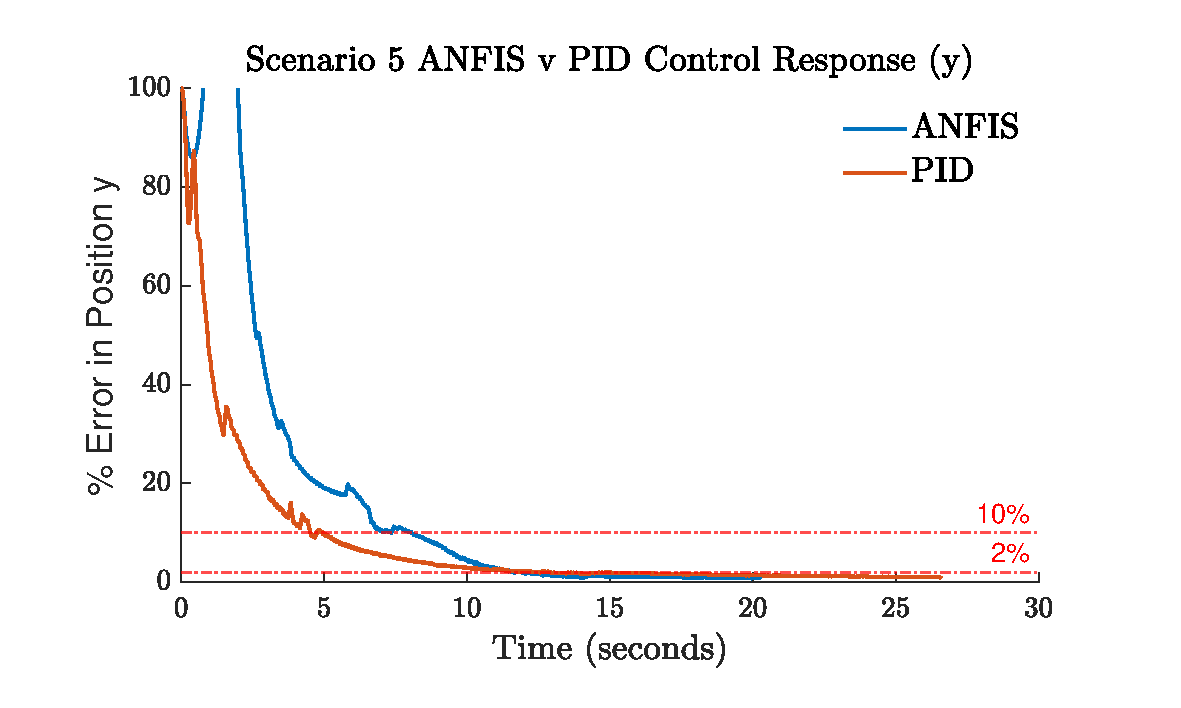
\includegraphics[height=5cm,keepaspectratio]{img/Scenario 5 Error in y Position.pdf}
        \caption{Scenario 5 Control Response (Error between Desired position $y$ and Actual position $y$) for PID and ANFIS Control}
        \label{fig:Response5y}
    \end{minipage}
\end{figure}

\begin{figure}[H]
    \centering
    \begin{minipage}[b]{0.45\textwidth}
        % empty minipage
    \end{minipage}
    \hfill
    \begin{minipage}[b]{0.45\textwidth}
        \centering
        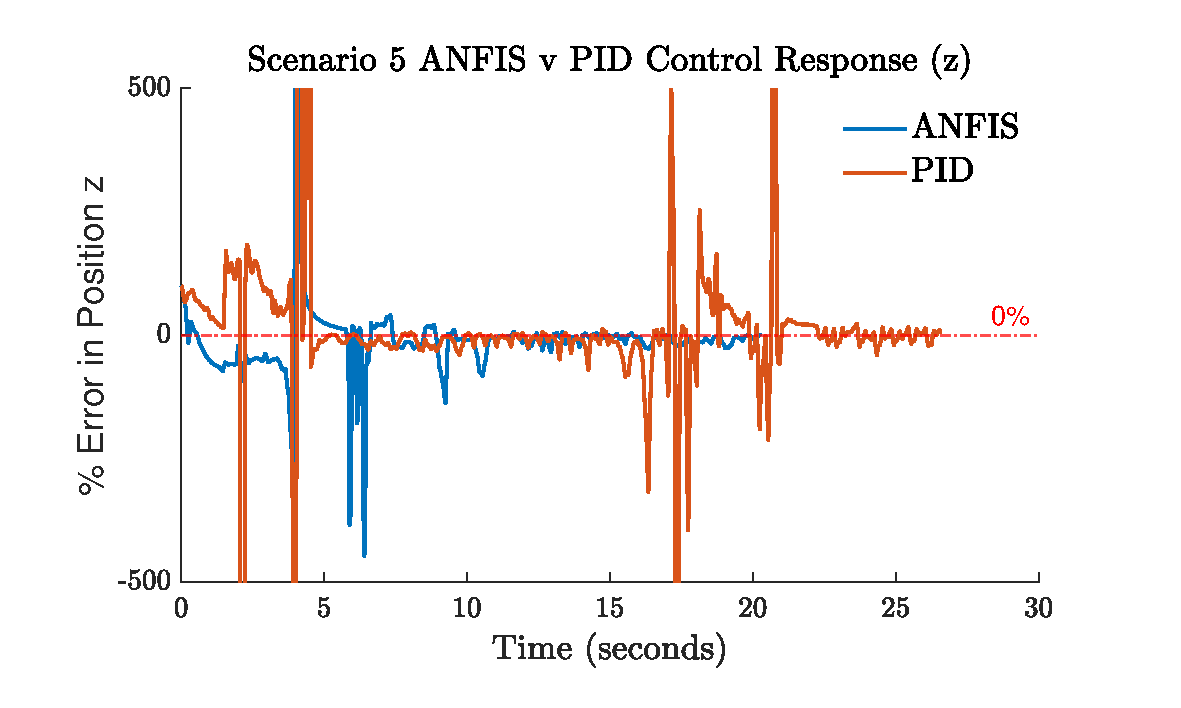
\includegraphics[height=5cm,keepaspectratio]{img/Scenario 5 Error in z Position.pdf}
        \caption{Scenario 5 Control Response (Error between Desired position $z$ and Actual position $z$) for PID and ANFIS Control}
        \label{fig:Response5z}
    \end{minipage}
    \hfill
    \begin{minipage}[b]{0.45\textwidth}
        % empty minipage
    \end{minipage}
\end{figure}

\subsection{Computational Power Results}
Computational power was simply evaluated for each scenario using the ``profiler'' functionality in MATLAB, giving a report on the peak and allocated computational memory used for the simulations, as well as the simulation time. As this measure could vary based on the computational device used, the same laptop under the same conditions (i.e. no other applications running on the device and laptop is on charge) and the average of five simulations in each case was taken. The machine used to collect the results was the AMD Ryzen 7 5800U with Radeon Graphics laptop, with a RAM of 8.00 GB (7.35GB usable). 

The results of the allocated memory and peak memory used for each scenario for both the ANFIS and PID controller are shown in Figures \ref{fig:alloc_memory} and \ref{fig:peak_memory}. Figure \ref{fig:peak_memory} shows that the peak memory used is very similar for all scenarios, with the ANFIS having a slightly higher peak memory usage in four out of the five scenarios. This indicates the ANFIS and PID controllers have similar peak computational requirements, however the ANFIS generally has a slightly higher maximum power requirement. 

Figure \ref{fig:alloc_memory} shows that the allocated memory used is higher for the ANFIS controller in all cases apart from Scenario 2. This may be because the control response was especially faster for this scenario, with the ANFIS controlled drone reaching its destination 29.2\% quicker than the PID. However in all the other scenarios, the ANFIS has a higher allocated memory. Scenario 4 shows a particularly higher allocated memory for the ANFIS controller, likely due to the worse control response discussed earlier. 
\begin{figure}[H]
    \centering
    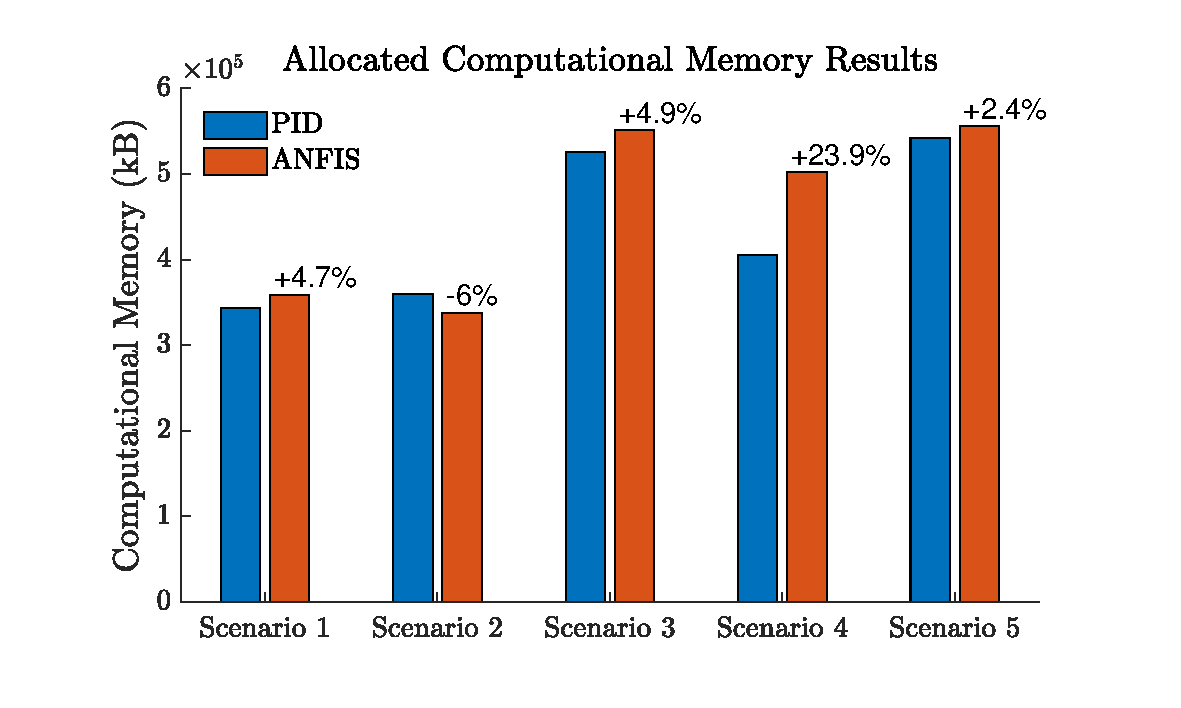
\includegraphics[width = 0.7\textwidth]{img/Allocated Computational Power.pdf}
    \caption{Allocated Computational Memory used by ANFIS and PID controllers for each scenario (labels show the difference in the value for ANFIS relative to the PID result)}
    \label{fig:alloc_memory}
\end{figure}
\begin{figure}[H]
    \centering
    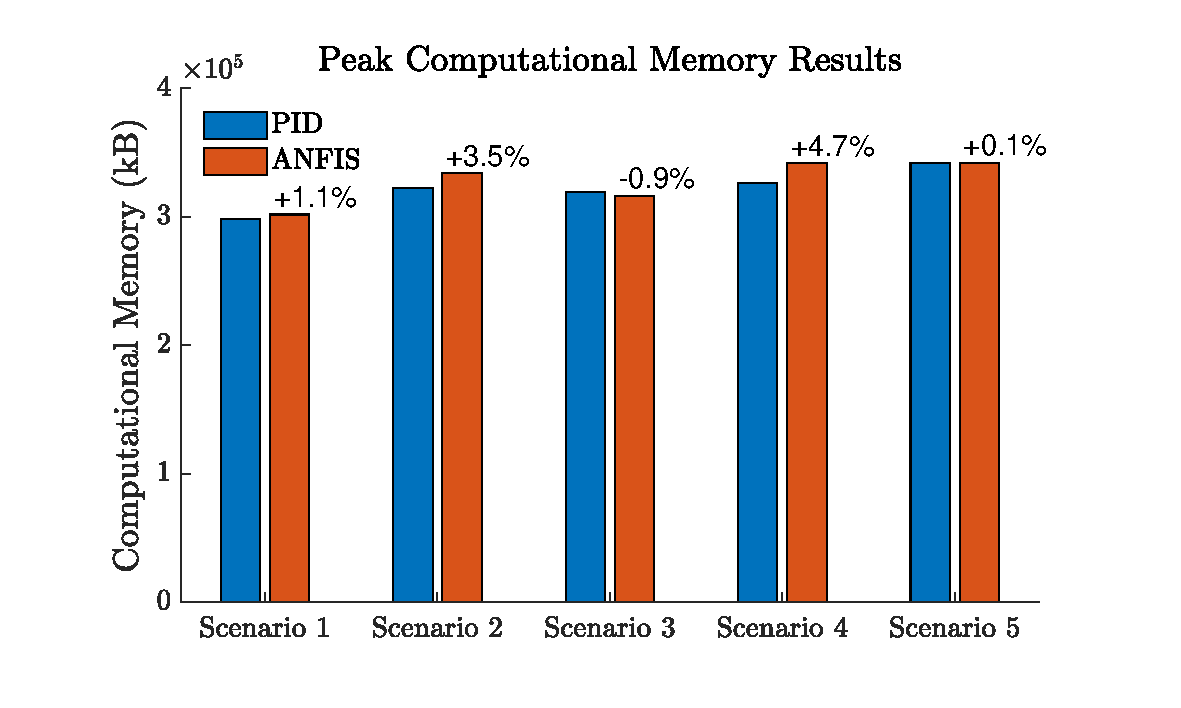
\includegraphics[width = 0.7\textwidth]{img/Peak Computational Power.pdf}
    \caption{Peak Computational Memory used by ANFIS and PID controllers for each scenario (labels show the difference in the value for ANFIS relative to the PID result)}
    \label{fig:peak_memory}
\end{figure}

The results for computational time, i.e. the actual time taken by the machine to perform the simulation (not be confused with the ``simulation time'' which is the time the drone takes to reach its destination) were also investigated for each scenario and are plotted in Figure \ref{fig:comp_time}. The results align with the findings from the control response apart from Scenario 1. In Scenarios 3 and 4 the ANFIS controller had a considerably higher computational time (46.8\% and 41.2\% respectively) which correlates with the slower control response in these scenarios. The ANFIS controller had a lower computational time than the PID controller in Scenarios 2 and 5, again analogous to the control response times. The ANFIS controller unusually had a slightly higher computational time in Scenario 1 which was against the trend scene in the other four scenarios. 

The computational memory results show that the ANFIS controller overall had a slightly higher computational memory usage and therefore is likely to require higher computational requirements. The rationale behind this could be due to the duality of the controller requiring increased computation. As a result of having to decide whether to use a PID or ANFIS response, the dual ANFIS controller uses more computational memory. This is supported by the computational time results correlating with the control response results and therefore the ANFIS controller having a shorter computational time for the scenarios with a relatively minimal change in height. 
\begin{figure}[H]
    \centering
    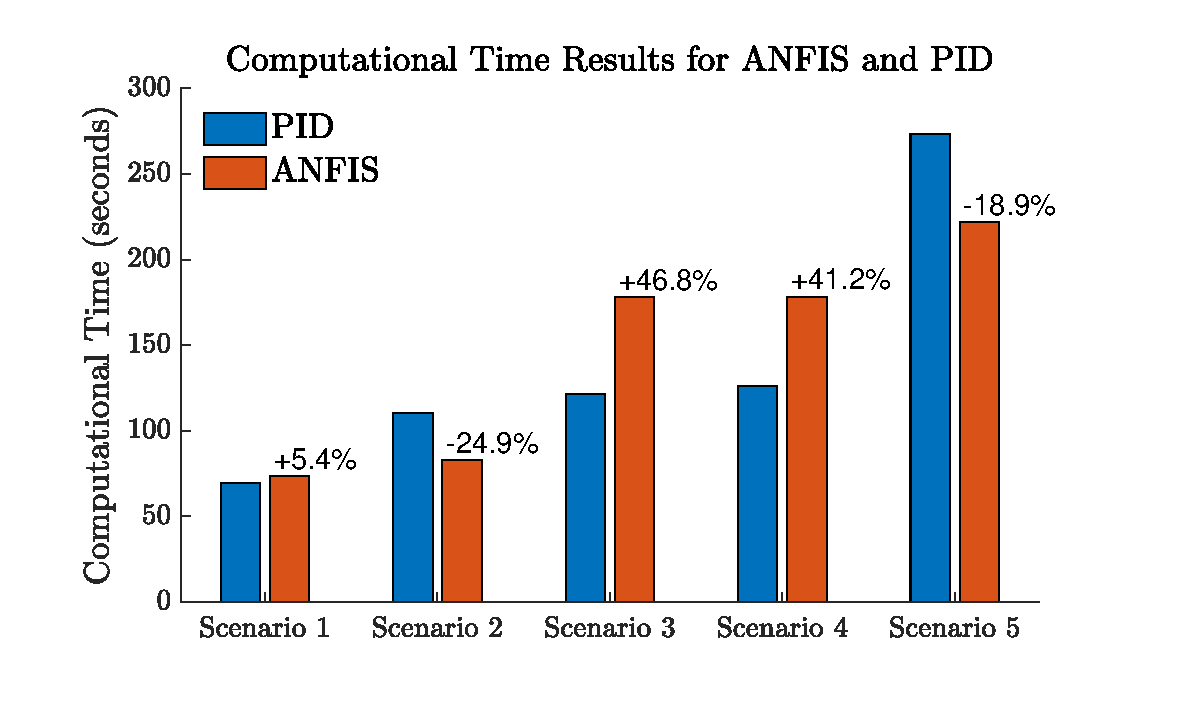
\includegraphics[width = 0.7\textwidth]{img/Computational Time.pdf}
    \caption{Computational Time taken by ANFIS and PID controllers for each scenario (labels show the difference in the value for ANFIS relative to the PID result)}
    \label{fig:comp_time}
\end{figure}